\documentclass[10pt]{article}


%Packages pour ecrire en fran�ais :
\usepackage[utf8]{inputenc}
\usepackage[T1]{fontenc}
\usepackage{lmodern}
\usepackage{numprint}
\npdecimalsign{.}
\nprounddigits{3}
\usepackage[english]{babel}
%Fin packages pour ecrire en fran�ais

%AU CHOIX 
\usepackage{MATISpdfhisto}
%\usepackage{MATISpdfupe}% page couverture et seconde page a facon

\usepackage{geometry} 
\usepackage{amstext,amsmath,amssymb}
\usepackage{color}
\usepackage{booktabs}
\usepackage[usenames,dvipsnames]{xcolor}

\PassOptionsToPackage{hyphens}{url}\usepackage[
colorlinks=true,
urlcolor=PineGreen,
linkcolor=RoyalBlue,
citecolor=blue
]{hyperref}

\usepackage{multirow}
\usepackage{geometry}
\usepackage{amsmath,amssymb}
\usepackage{amsmath}
\usepackage{amsfonts}
\usepackage{csquotes}
\usepackage{pgffor}
\usepackage{amssymb}
\usepackage{chngcntr}
\usepackage{mathtools}
\usepackage{slashbox}

\newcommand{\exposantdevant}[1][2]{\prescript{##1}{}{##2}}
\newcommand{\indicedevant}[1][2]{\prescript{}{##1}{##2}}
\newcommand{\transpose}[1]{\prescript{t}{}{##1}}
\DeclareMathOperator{\atan}{atan}
\DeclareMathOperator{\sgn}{sgn}
\DeclareMathOperator{\abs}{abs}
\DeclareMathOperator{\argmax}{argmax}
\DeclareMathOperator{\argmin}{argmin}
\usepackage{algorithm}
\usepackage[noend]{algpseudocode}
\makeatletter
\def\BState{\State\hskip-\ALG@thistlm}
\makeatother

\usepackage{cellspace}
\usepackage{slashbox}
\usepackage{pdfpages}
\usepackage{enumitem}
\usepackage[pdftex]{graphicx}
\usepackage{subcaption}
\graphicspath{{Figures/}{Figures/finistere_T41000_30000/}{Figures/finistere_T35000_40000/}{Figures/gironde_T10500_34500/}{Figures/finistere_all/}}

%Bibliography
\usepackage[
backend=biber,
style=authoryear,
citestyle=authoryear,
uniquename=init,
maxcitenames=1,
giveninits=true,
hyperref=auto,
sorting=nyt
]{biblatex}
\addbibresource{rapport.bib}


\newcommand{\wbal}{The Wikibook about \LaTeX}
\newcommand{\legende}{\vspace{3mm}
    
    \small\centering
    \fcolorbox{black}{red}{\rule{0pt}{6pt}\rule{6pt}{0pt}}\quad Building \hspace{2mm} \fcolorbox{black}{gray}{\rule{0pt}{6pt}\rule{6pt}{0pt}}\quad Road \hspace{2mm}
    \fcolorbox{black}{green}{\rule{0pt}{6pt}\rule{6pt}{0pt}}\quad Forest \hspace{2mm}
    \fcolorbox{black}{yellow}{\rule{0pt}{6pt}\rule{6pt}{0pt}}\quad Other Vegetation \hspace{2mm}
    \fcolorbox{black}{blue}{\rule{0pt}{6pt}\rule{6pt}{0pt}}\quad Water
    }
    
\newcommand{\legendeBinEval}{\vspace{3mm}
    
    \small\centering
    \fcolorbox{black}{green}{\rule{0pt}{6pt}\rule{6pt}{0pt}}\quad Good \hspace{2mm}
    \fcolorbox{black}{red}{\rule{0pt}{6pt}\rule{6pt}{0pt}}\quad Bad (GT=1) \hspace{2mm}
    \fcolorbox{black}{blue}{\rule{0pt}{6pt}\rule{6pt}{0pt}}\quad Bad (Classification=1)
    }
    
\newcommand{\legendebuf}{\vspace{3mm}
    
    \small\centering
    \fcolorbox{black}{red}{\rule{0pt}{6pt}\rule{6pt}{0pt}}\quad Building \hspace{2mm} \fcolorbox{black}{gray}{\rule{0pt}{6pt}\rule{6pt}{0pt}}\quad Road \hspace{2mm}
    \fcolorbox{black}{green}{\rule{0pt}{6pt}\rule{6pt}{0pt}}\quad Forest \hspace{2mm}
    \fcolorbox{black}{yellow}{\rule{0pt}{6pt}\rule{6pt}{0pt}}\quad Other Vegetation \hspace{2mm}
    \fcolorbox{black}{blue}{\rule{0pt}{6pt}\rule{6pt}{0pt}}\quad Water\hspace{2mm}
    \fcolorbox{black}{cyan}{\rule{0pt}{6pt}\rule{6pt}{0pt}}\quad Buffer Class
    }
    
\newcommand{\legendebin}{\vspace{3mm}
    
    \small\centering
    \fcolorbox{black}{red}{\rule{0pt}{6pt}\rule{6pt}{0pt}}\quad Artificialized area 
    \fcolorbox{black}{green}{\rule{0pt}{6pt}\rule{6pt}{0pt}}\quad Non-artificialized area
    }
\newcommand{\tile}{41000_30000}    
\newcommand{\region}{finistere}

\MATISdate{\today}
\MATISdatee{\today}

\MATISauthor{Cyril Wendl}                                                          
\MATISauthore{Cyril \textsc{Wendl}}
\MATISauthormail{cyril.wendl@epfl.ch}
\authorhead{Cyril \textsc{Wendl}}

\titlehead{Fusion of Multi-Temporal Sentinel-2 image Series and Very-High Spatial Resolution Images for Detection of Urban Areas}

\MATISetitle{Fusion of Multi-Temporal Sentinel-2 image Series and Very-High Spatial Resolution Images for Detection of Urban Areas}

%\MATISaffiliation{IGN - Laboratoire MATIS, CRNI - Strasbourg, EPFL}
\MATISaffiliatione{IGN - Laboratoire MATIS, CRNI - Strasbourg, EPFL}
%Supervisors: Arnaud Le-Bris (IGN), Anne Le-Puissant (CRNI), Frank De Morsier (EPFL)
%\MATISaffiliationune{IGN - Laboratoire MATIS}


%%%%%%%%%%%%%%%%%%%%%%%%
%  Resume & abstract
%%%%%%%%%%%%%%%%%%%%%%%%

%\MATISresume{Summary}
%\MATISmotcle{}
\MATISabstract{Fusion of very high spatial resolution multispectral images with lower spatial resolution image time series having a higher number of bands can enable better land use classification, combining geometric and semantic advantages of both sources. This study presents a workflow to find the extent of urbanized ground using decision-level fusion and regularization at the pixel level of Sentinel-2 and SPOT-6 satellite images. First, both images are classified individually in five classes, using state-of-the-art supervised classification approaches and neural networks. Decision-level fusion and regularization are used for combining the spatial and spectral advantages of both classifiers: First, both sources are merged such as to extract building labels with as high semantic and spectral precision as possible. Second, this product together with the Sentinel-2 classification are used as \textit{a priori} input for a binary classification of the artificialized area. The building labels from the regulation are dilated in order to connect the building objects and a binary classification is derived from the original Sentinel-2 classification. These binary classifications are reintroduced in a fusion and regularization to find the artificialized area. Segmentation of the Sentinel-2 satellite image and majority voting of the object-level classification are used to refine the contours of the artificialized area.}

\MATISkeyword{Decision fusion, Regularization, Urban classification, Multispectral, Urban patch, Artificialization}

%%%%%%%%%%%%%%%%%%%%%%%%%%%%%%%%%%%%%%%%%
%       FIN DE LA PRESENTATION
%%%%%%%%%%%%%%%%%%%%%%%%%%%%%%%%%%%%%%%%%

%%%%%%%%%%%%%%% Debut du rapport a proprement parle %%%%%%%%%%%%%%%
\begin{document}

%%%% On importe le style
\makeMATIS

%%%% Apres, c'est comme d'habitude, on ne change rien. %%%%

\tableofcontents
\newpage
\section{Introduction}
% Importance of ground occupation classification: urban spread, planning

% Fusion: combination of high spectral and spatial resolution
Classification of urban land cover is of central importance to monitor urban sprawl, impermeabilization of soils and to predict their further evolution (\cite{kurtz_histogram_2012,kurtz_extraction_2012,wemmert_multiresolution_2009}). Supervised classification approaches using satellite imagery have been studied to automate the process of land use classification to a certain degree  \parencite{inglada_operational_2017,li_urban_2016}. High spatial resolution satellite images enable the delineation of much smaller features, however they are often characterized by semantic uncertainty that is, not having enough spectral information to distinguish land cover types precisely, resulting in confusion of classes. On the other hand, satellites using many bands offer high spectral depth offering more semantic information but less geometric detail. Fusion of several sources aims at combining their advantages to reduce spatial and semantic uncertainties \parencite{ouerghemmi_two-step_2017,fauvel_decision_fusion,hervieu_fusion_2016}. \\

% Fusion at decision level
Fusion schemes can be regrouped on three levels \parencite{ouerghemmi_two-step_2017}:
\begin{enumerate}
    \item At the data level, where the original images are merged, using methods such as pan-sharpening of the multispectral image in order to produce the best single classification;
    \item At the feature level, applying a single classification to extract features from both sources;
    \item At the decision level, where two separate classifications from heterogeneous data sets are merged.
\end{enumerate}

\cite{ouerghemmi_two-step_2017} have proposed several fusion approaches at decision level as well as a regularization whose aim is to smooth the fusion result while using the contrast information of the original image to follow the object contours and reinforce the geometric accuracy after the fusion. \\

% Aim
The aim of this paper is to propose a decision-level fusion processing chain using freely available and commercial satellite imagery to improve the automatic ground use classification in urban environments in the following five categories: building, roads, water, forest and other vegetation. Firstly, a ground classification map is produced following as precisely as possible the contours of individual buildings and roads. Secondly, this product is used as an \textit{a priori} input data set for the derivation a binary land use map of the "urban footprint", which can be understood as the area made irreversibly impermeable through the construction of buildings and roads, including smaller enclosed structures such as backyards \parencite{puissant_object-oriented_2014}. This bigger aggregation of buildings, roads and enclosed small structure will be called hereafter "artificialized area" or "urban footprint".\\

The aim of this study is twofold:
\begin{enumerate}
    \item To provide an accurate classification of buildings and roads using decision-level fusion of Sentinel-2 and SPOT-6 classifications;
    \item To produce a map of the artificialized area using the result of the previous fusion. 
\end{enumerate}

% data sources
\subsection{Satellite data and Study Sites}
The satellite data used for the ground land classification are described in in tables \ref{table:bands_s2} and \ref{table:bands_spot}.
\begin{table}[H]
    \centering
    \begin{subtable}{.52\textwidth}
        \centering
        \begin{tabular}{@{}lp{2cm}p{2.2cm}l@{}}\toprule
            Band & Resolution [m] & Central Wavelength [nm] & Domain \\\hline
            B1 & 60 & 443 & Violet \\
            B2 & 10 & 490 & Blue \\
            B3 & 10 & 560 & Green \\
            B4 & 10 & 665 & Red \\
            B5 & 20 & 705 & VNIR \\
            B6 & 20 & 740 & VNIR \\
            B7 & 20 & 783 & VNIR \\
            B8 & 10 & 842 & VNIR \\
            B8a & 20 & 865 & VNIR \\
            B9 & 60 & 940 & SWIR \\
            B10 & 60 & 1375 & SWIR \\
            B11 & 20 & 1610 & SWIR \\
            B12 & 20 & 2190 & SWIR\\\bottomrule
        \end{tabular}
        \caption{Sentinel-2 Level 2A (\cite{esa-s2res,theia})}
        \label{table:bands_s2}
    \end{subtable}
    \begin{subtable}{.45\textwidth}
        \centering
        \begin{tabular}{@{}lp{1.7cm}p{2.1cm}l@{}}\toprule
            Band & Resolution after pan-sharpening [m] & Wavelength range [nm] & Domain \\\hline
            B0 & 1.5 & 450 - 520 & Blue \\
            B1 & 1.5 & 530 - 590 & Green \\
            B2 & 1.5 & 625-695 & Red \\
            B3 & 1.5 & 760-890 & VNIR \\\bottomrule
        \end{tabular}
        \caption{SPOT-6 (\cite{SPOT6_technical-sheet})}
        \label{table:bands_spot}
    \end{subtable}
    \caption{Spatial and spectral resolution of satellite data. VNIR = Visible and Near Infrared, SWIR = Short Wave Infrared}
    \label{table:bands}
\end{table}
Regarding Sentinel-2, only the 10 bands having a resolution of 10 or 20 meters were used and in practice the bands having a resolution of 20 meters were up-scaled to 10 m resolution. Regarding SPOT-6, the resolution was obtained by using a fifth monochromatic band for pan-sharpening. \\

Sentinel-2 data was downloaded on several dates in order to mitigate seasonal effects on land cover classification. Table \ref{table:dates} lists the used dates for each satellite and test region.
\begin{table}[H]
\centering
\begin{tabular}{lll}\toprule
Region & Sentinel-2 dates & SPOT-6 dates \\\hline
\multirow{5}{*}{Finistère} & 2017-05-25 & \multirow{5}{*}{2014-04-16} \\
 & 2017-04-12 &  \\
 & 2017-03-16 &  \\
 & 2017-01-25 &  \\
 & 2016-08-15 &  \\\hline
\multirow{4}{*}{Gironde} & 2017-06-18 & \multirow{4}{*}{2016-03-22} \\
 & 2017-04-19 &  \\
 & 2016-11-30 &  \\
 & 2016-09-01 &  \\\bottomrule
\end{tabular}
\caption{Used dates for each classification}
\label{table:dates}
\end{table}
% TODO pq on a pris des dates très similaires pour la Finistère ? date 2016 ?

All classifiers presented below have been applied to a zone spanning in the Finistère region in North-Western France and Gironde in Western France near Bordeaux. Fusion and regularization products are produced for the entire zone covered in both available datasets for Finistère, spanning 648 $km^2$. Results are presented visually for a sub-zone of 0.64 $km^2$ area (fig.  \ref{fig:area\tile}).
\newcommand{\figureTile}{
\begin{figure}[H]
    \centering
    \begin{subfigure}{0.49\textwidth}
        \centering
        \includegraphics[width=.9\textwidth]{\region_T\tile_Im_SPOT6}
        \caption{SPOT 6 image tile (3000$\times$ 3000 m)}
    \end{subfigure}
    \hfill
    \begin{subfigure}{0.49\textwidth}
        \centering
        \includegraphics[width=.9\textwidth]{\region_T\tile_Im_SPOT6_crop}
        \caption{Zoomed area (800 $\times$ 800 m)}
    \end{subfigure}
    \caption{SPOT6 image tile and crop window used for visualization in the report}
    \label{fig:area\tile}
    \centering
\end{figure}
}
\figureTile

\section{Methodology}\label{sec:method}
\subsection{Workflow}
Figure \ref{fig:methods} shows the overall workflow for producing a classification based on fusion, regularization as well as the second classification using the Sentinel2 image, illustrating all the above-mentioned steps. The fusion method producing the best results in terms of visual quality, absence of artifacts and accuracy measures was retained and used further in the Regularization step. Several regularization parameters mentioned above were tested and the set of parameters producing the best map was retained, in terms of its visually appealing properties, truthfulness to real-world objects and classification accuracies.

\begin{figure}[H]
    \centering
    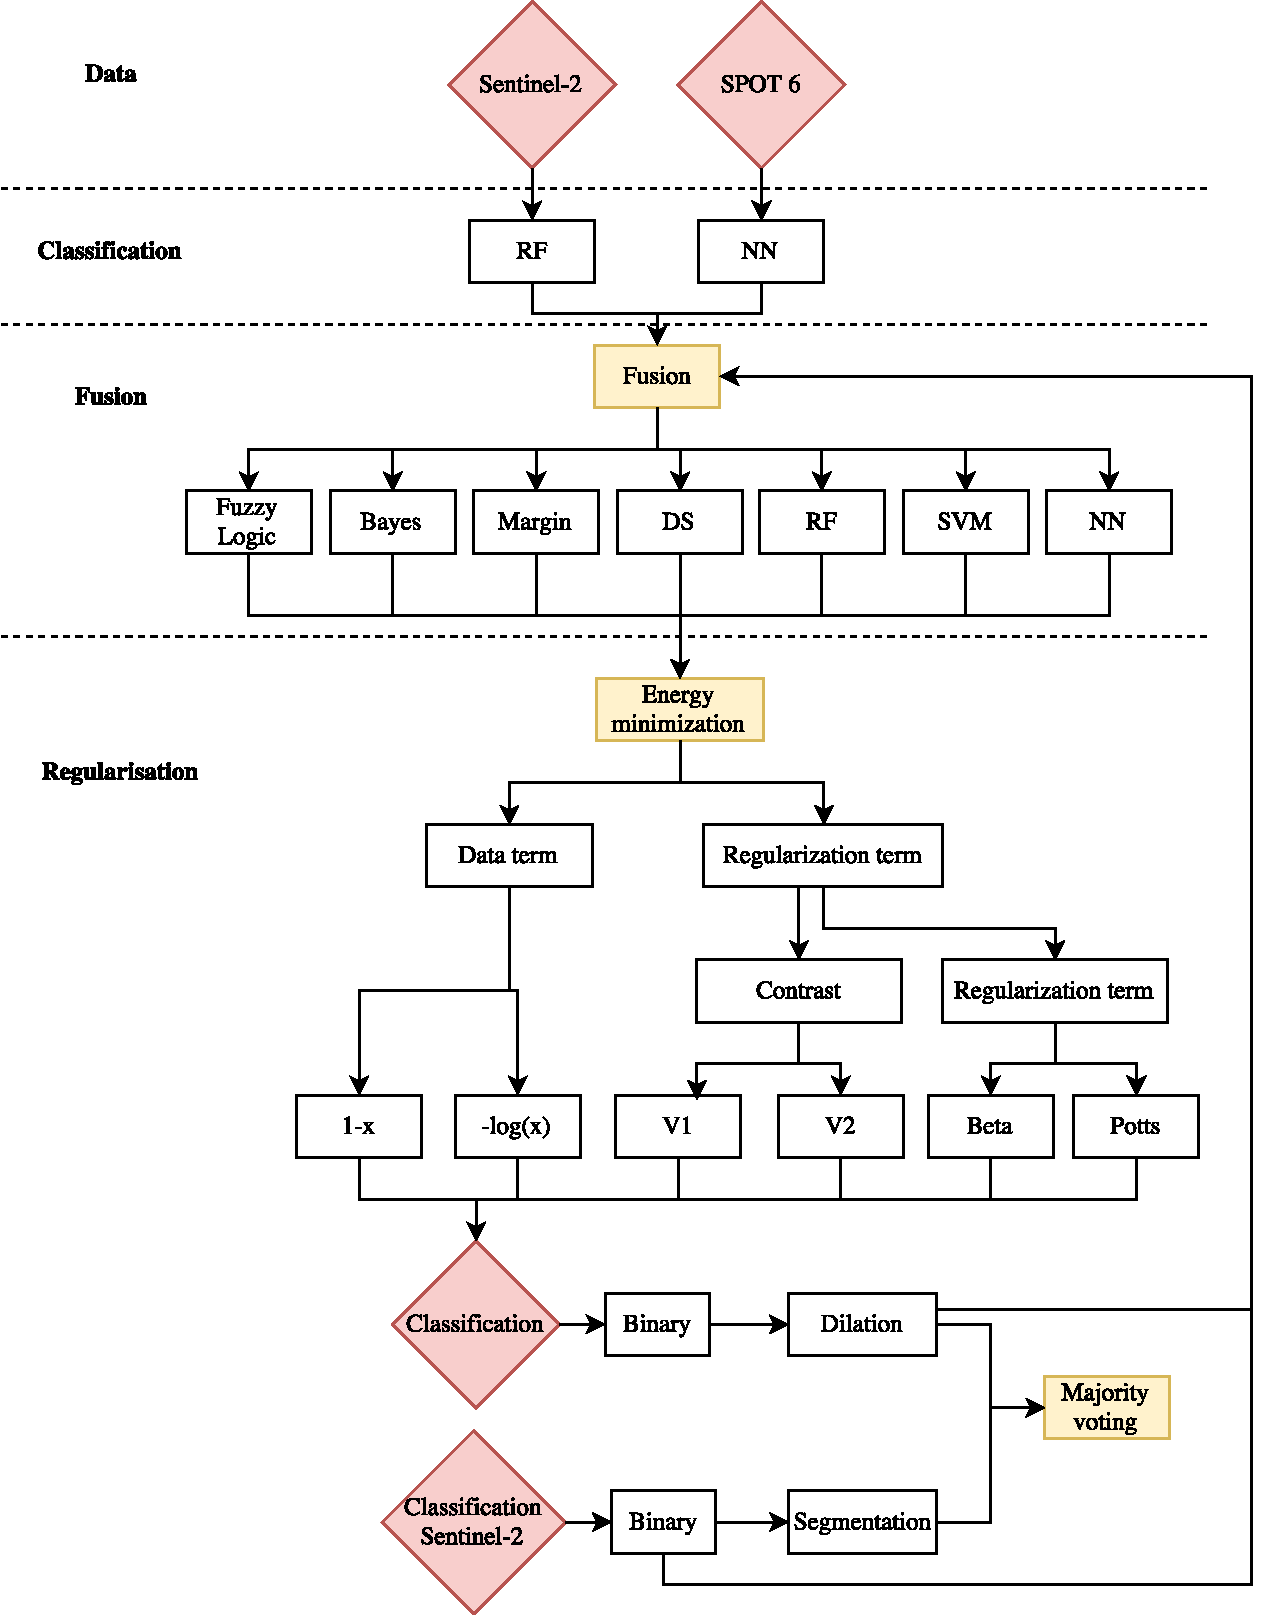
\includegraphics[width=.7\textwidth]{IGN-methods}
    \caption{Methods}
    \label{fig:methods}
\end{figure}
\subsection{Initial Fusion}

The data sets were first classified individually before fusion: The Sentinel-2 image was classified using 10 bands of each date (tables \ref{table:bands_s2}, \ref{table:dates}) using a Random Forest classifier with 50'000 samples per class and 100 trees \parencite{Breiman2001}. The SPOT-6 image was classified using a Deep Convolutional Neural Network (DCNN) on the four bands of the SPOT-6 image descripbed in tables \ref{table:bands_spot}, \ref{table:dates} (\cite{postadjian_investigating_2017}). Both classifiers produced membership probabilities for the 5 classes described in the introduction (building, roads, water, forest and other vegetation).\\

The Random Forest classifier was trained using ground truth data of the freely available BDTOPO and RPG databases, from which a ground truth map of 5 class labels was derived (\cite{bdtopo,RPG}, fig. \ref{fig:vt\tile}).
\newcommand{\figureGT}{
\begin{figure}[H]
    \centering
    \begin{subfigure}{0.49\textwidth}
        \centering
        \includegraphics[width=\textwidth]{\region_T\tile_Im_SPOT6_crop}
        \caption{Original image (SPOT 6)}
        \label{fig:SPOT6\tile}
    \end{subfigure}
    \begin{subfigure}{0.49\textwidth}
        \centering
        \includegraphics[width=\textwidth]{\region_T\tile_train}
        \caption{Ground Truth}
        \label{fig:GT\tile}
    \end{subfigure}
    \legende
    \caption{Original image and ground truth. Black parts indicate missing ground truth data.}
    \label{fig:vt\tile}
\end{figure}
}
\figureGT

\subsection{Fusion schemes}\label{sec:fusion}
% TODO Notation
% TODO Explain better: Compromis WO, DS MasseSomme, DS MasseV1, Marge Bayes Pond / Marge Max / Marge Somme Pond / Moyenne  Bayes=Prod, Somme=Bayes Somme, CompromisWO=Walid Ouerghemmi

The fusion rules presented below are based on previous work by \cite{ouerghemmi_two-step_2017} and propose pixel-level decision schemes between two or more classifiers based on their class membership probabilities.
\subsubsection{Fuzzy Rules}\label{sec:fuzzyLogic}
The first tested fusion approach is based on fuzzy rules \cite{zadeh_fuzzy_1965}. Fuzzy rule theory states that a fuzzy set $\mathcal{A}$ in a reference set $\mathcal{L}$ is a set of ordered pairs:
\begin{equation}
    A=[(x,P_A(x)|x\in \mathcal{L})]
\end{equation}
Where the membership probability of $A$ in $\mathcal{P}$ is given by $P_A:\mathcal{L}\rightarrow[0,1]$.

The measure of conflict between two sources ($1-K$) is given as (\cite{ouerghemmi_two-step_2017,dubois_possibility}):
\begin{equation}
    K=\sup_x\min(P_A(x), P_B(x))
\end{equation}
In order to account for the fact that fuzzy sets with a strong fuzziness possibly hold unreliable information, each fuzzy set $i$ is weighted by a pointwise confidence measure $w_i$ as proposed by \cite{fauvel_decision_fusion}:
\begin{equation}
    w_i=\frac{\sum_{k=0,k\neq i}^{n}H_{\alpha QE}(P_k)}{(n-1)\sum_{k=0}^{n}H_{\alpha QE}(P_k)}
\end{equation}
$n$ being the number of sources and $H_{\alpha QE}$ a fuzziness measure called $\alpha$-quadratic entropy (QE) \parencite{pal_measuring_1994}. Every fuzzy set $i$ is weighted by the fuzziness degree of all other fuzzy sets (classifications) $k\in n,k\neq i$. If the fuzziness degree of the other sets is high the weight on a given source $i$ will be high too. For all of the following fusion rules, the fuzzy sets have been weighted as $\tilde{P}_A(x)=w_A\cdot P_A(x), \tilde{P}_B(x)=w_B\cdot P_B(x)$, $P_A(x)$ and $P_B(x)$ being the original membership probabilities and $w_A, w_B$ their corresponding pointwise measures.\\

All fuzzy rules have been tested using the original class probabilities as input  as well as using the probabilities weighted by the pointwise measure of their fuzziness degree (section \ref{sec:fuzzyLogic}). The hypothesis was that weighting the probabilities by their fuzziness could help improve other fusion methods as well by reducing the importance of fuzzy sources. In fig. \ref{fig:proba_point}, an example is shown where the SPOT 6 classifier has a higher fuzziness degree than the Sentinel-2 classifier, hence the probability of the SPOT 6 classifier is reduced more strongly by the pointwise measure.
\begin{figure}[H]
    \centering
    \includegraphics[width=.7\textwidth]{\region_T\tile_proba_point}
    \caption{Original and weighted class probabilities}
    \label{fig:proba_point}
\end{figure}

The following fusion rules based on fuzzy logic were considered:
\begin{enumerate}
    \item Minimum rule as the intersection of two fuzzy sets $P_A$ and $P_B$, given by the minimum of their membership probabilities (conjunctive behaviour):
    \begin{equation}
        \forall A\in\mathcal{L} \;\;\; (P_A\cap P_B)(x) = P_{fusion}(x) =\min\big(P_A(x),P_B(x)\big)
    \end{equation}
    \item Maximum rule as the union between the two fuzzy sets $P_A$ and $P_B$, given by the maximum of their membership probabilities (disjunctive behaviour):
    \begin{equation}
        \forall A\in\mathcal{L} \;\;\; (P_A\cup P_B)(x) = P_{fusion}(x)=\max\big(P_A(x),P_B(x)\big)
    \end{equation}
    \item Compromise operator:
    \begin{equation}\label{eq:compro}
        P_{fusion}(x)=
        \begin{cases}
            \max\Big(T_1,\min\big(T_2,(1-K)\big)\Big)& \text{if } (1-K)\neq q\\
            \max\Big(P_A(x),P_B(x)\Big) &\text{if }(1-K)= 1
        \end{cases}
    \end{equation}
    where $T_1=\frac{\min\big(P_A(x),P_B(x)\big)}{K}$ and $T_2=\max\big(P_A(x),P_B(x)\big)$, noticing that the operator behavior is conjunctive when the conflict between $A$ and $B$ is low ($1-K\approx 0$) and disjunctive when the conflict is high ($1-K\approx 1$). When the conflict is partial, the operator behaves in a compromise way \parencite{ouerghemmi_two-step_2017}. This fusion approach would however favour $T_1$ at fusion level, therefore \cite{ouerghemmi_two-step_2017} propose to measure the intra-class conflict as $f_c=\abs(Cbest1-Cbest2)$ and set a conflict threshold $t_c=0.25$ to be used as follows:
    
    \begin{algorithm}[H]
        \begin{algorithmic}
            \If {$f_c<t_c$} 
            \Comment{existence of intra-membership conflict}
            \State $P_{fusion}=\max\big(P_A(x),P_B(x)\big)$
            \Else
            \Comment{no intra-membership conflict}
            \State $P_{fusion}$ following equation \ref{eq:compro}
            \EndIf
        \end{algorithmic}
        \caption{Compromise rule according to \cite{ouerghemmi_two-step_2017}}
        \label{alg:comp-wo}
    \end{algorithm}
    \item Prioritized operators (Prior 1, eq. \ref{eq:prior1} and Prior 2, eq. \ref{eq:prior2}):
    \begin{align}
        P_{fusion}(x)&=\max\big(P_A(x),\min(P_B(x),K)\big)\label{eq:prior1}\\
        P_{fusion}(x)&=\min\Big(P_A(x),\max\big(P_B(x),(1-K)\big)\Big)\label{eq:prior2}
    \end{align}
    If the conflict between $A$ and $B$ is high (i.e., $K\approx 0$), only $P_A$ is taken into account (prioritized) and $P_B$ is considered a a specific piece of information. Thus, the fusion result will depend on the order of the classes $A$ and $B$.
\end{enumerate}

\subsubsection{Bayesian combination}\label{sec:bayesian}
A very simple approach is to sum or multiply the input probabilities as a Bayesian sum or product:
\begin{align}
    P_{fusion}&=P_A(x)+P_B(x)\\
    P_{fusion}&=P_A(x)\times P_B(x)
\end{align}
Those fusion rules will be referred to as Bayesian Sum and Bayesian Product. Both were weighted by the margin. % TODO clarify
\subsubsection{Margin-based Rule (Margin-Max)}\label{sec:margin}
In the Max-Margin approach, the aim is to conserve the most confident source in each pixel, that is, the one having the least smallest margin:
\begin{equation}
    margin^{(s)}(x)=P_s^{cbest1}-P_s^{cbest2}(x)
\end{equation}
where $cbest1=\argmax_{c\in\mathcal{L}}P_S(C)$ and $cbest2=\argmax_{c\in\mathcal{L}\setminus cbest1}P_S(C)$. The fusion will choose for each pixel the source for which the margin between the two highest probabilities is the biggest, with sources $\mathcal{S}={A,B}$ and the classes $\mathcal{L}=\{\mathcal{C}_i\}_{i\in[1,n]}$:
\begin{equation}
    \forall x,\forall c\in \mathcal{L}\;\;\; P_{fusion}^{(c)}(x)=P_{S_{best}}^{(c)}(x)
\end{equation}
where $S_{best}=\argmax_{\mathcal{S}\in\mathcal{C}}margin^{(s)}(x)$.


\subsubsection{Dempster-Shafer (DS) evidence theory}\label{sec:DS}
According to the DS formalism, an information from a source $s$ for a class $c$ can be given as a mass function $m_c\vert m_c\in [0,1]$ (\cite{shafer-evidence}). Dempster-Shafer's evidence theory rule assumes simple classes $c\in \mathcal{L}$ as well as composed classes, which were limited to at most two simple classes as indicated in \cite{ouerghemmi_two-step_2017}. Masses associated to each simple class were denoted as taking simply the class membership probability.
\begin{align}
    m_s^{(c)}(x)=P_s^{(x)}
\end{align}
For compound classes, $\forall c_1,c_2\in \mathcal{L}, \forall$ pixel $x$ and $\forall s\in \mathcal{S}$, two versions were tested, denoted $V_1$ and $V_2$, respectively
\begin{align}
    m_s^{(c_1\cup c_2)}(x)&=\big(P_s^{(c_1)}(x)+P_s^{(c_2)}(x)\big)\times \Big(1-\max\big(P_s^{(c_1)}(x),P_s^{(c_2)}(x)\big)\Big)+\min\big(P_s^{(c_1)}(x),P_s^{(c_2)}\big)\\
    m_s^{(c_1\cup c_2)}(x)&=\frac{1}{2}\big(P_s^{(c_1)}(x)+P_s^{(c_2)}(x)\big)\times \Big(1-\max\big(P_s^{(c_1)}(x),P_s^{(c_2)}(x)\big)\Big)+\min\big(P_s^{(c_1)}(x),P_s^{(c_2)}\big)
\end{align}
This yields a mass $m_s^{(c_1\cup c_2)}(x)\in [0,1]$ being 1 if $P_s^{(c_1)}=0, P_s^{(c_2)}=1$ or $P_s^{(c_2)}=0, P_s^{(c_1)}=1$. In both versions, all masses are normalized such that $\sum_{c \in \mathcal{L}}^{(s)}m_c^{(s)}(x)=1$.
The fusion rule is based on the following conflict measure between two sources $A$ and $B$:
\begin{align}
    K(x)=\sum_{\substack{c,d\in\mathcal{L}'\\c\cap d\neq\emptyset}}^{(s)}=m_A^{(c)}(x)m_B^{(c)}(x)
\end{align}
$c,d\in\mathcal{L}$ being compound classes with $c\cap d =\emptyset$. The fusion is performed as:
\begin{equation}
    m_{fusion}^{(c)}(x)=\frac{1}{1-K(x)}\sum_{\substack{c_1,c_2\in\mathcal{L}'\\c_1 \cap c_2 = c}}^{(s)}m_A^{(c)}(x)m_B^{(c)}(x)
\end{equation}

\subsubsection{Fusion by Classification}
Supervised Classification Methods were used to perform a fusion on decision level. Following models were trained on the ground truth derived from the BDTOPO and RPG databases (\cite{bdtopo,RPG}), using the LIBSVM and OpenCV libraries (\cite{libsvm,opencv}) :
\begin{enumerate}
    \item Random Forest (RF), with 10'000 training samples per class and 100 trees (\cite{opencv})
    \item Support Vector Machine (SVM) with a linear kernel ($u'\times v$), with 10'000 training samples per class (\cite{libsvm})
    \item SVM with a radial basis kernel function: $\exp(-\gamma*|u-v|^2)$, with 500 training samples per class (\cite{libsvm}). Parameters of the SVM model were optimized using cross-validation. % TODO cite
\end{enumerate}
Each classifier was trained using the ground truth from the BDTOPO and RPG databases \cite{bdtopo,RPG}. Since the ground truth could contained gaps between buildings, the classifiers tended to aggregate individual buildings as there was no training data available around building. A sixth arbitrary buffer class extending 10 m radius around each building was added to the ground truth to preserve more details of the buildings during classification (fig. \ref{fig:vt_buffer}). Since only building labels were extracted for the subsequent steps, the other class labels as well as the buffer label could be ignored.

\begin{figure}[H]
    \centering
    \begin{subfigure}{0.49\textwidth}
        \centering
        \includegraphics[width=\textwidth]{\region_T\tile_train_5cl}
        \caption{Original Ground Truth}
        \label{fig:GT_5cl}
    \end{subfigure}
    \begin{subfigure}{0.49\textwidth}
        \centering
        \includegraphics[width=\textwidth]{\region_T\tile_train}
        \caption{Ground Truth with filled-in gaps}
        \label{fig:GT_6cl}
    \end{subfigure}
    \legendebuf
    \caption{Ground truth with buffer class}
    \label{fig:vt_buffer}
\end{figure}


\subsection{Regularization}\label{sec:regularization}
In order to smooth the fusion result, which still contains noisy patches, and make it follow real-world contours more accurately, an energy minimization regularization function was applied based on previous work by \cite{hervieu_fusion_2016} and \cite{ouerghemmi_two-step_2017}. The regularization consists of two terms, one related to the data fidelity, and one to the spatial regularization respectively:

\begin{equation}
    E(P_{fusion},C_{fusion},C)=\sum_{x\in I_{MS}}E_{data}(C(x))+\lambda\sum _{\substack{x,y\in N\\x\neq y}}E_{reg}(C(x),C(y))
\end{equation}
where:
\begin{equation*}
    \begin{aligned}
    E_{data}\big(C(x)\big)&=f\Big(P_{fusion}C(x)\big)\Big)\\
    E_{reg}\big(C(x)=C(y)\big)&=g\Big(P_{fusion}\big(C(x)\big),C_{fusion}\Big)\\
    E_{reg}\big(C(x)\neq C(y)\big)&=h\Big(P_{fusion}\big(C(x)\big),C_{fusion}\Big)
    \end{aligned}
\end{equation*}
    
The data term is a fit-to-data attachment term which models the probability distribution $P_{fusion}$. defined by a function $f(t)$. Following options were tested:
\begin{align}
\text{Option 1: } f(t)&=-\log(x)\\
\text{Option 2: } f(t)&=1-x
\end{align}
The regularization term $E_{reg}$ is based on a enhanced Potts model (\cite{schindler_overview_2012}) to prefer smoother label changes . A simple Potts model is defined as:
\begin{equation}
    \begin{aligned}
        E_{reg}(C(x)=C(y)&=0\\ 
        E_{reg}(C(y)\neq C(y))&=1
    \end{aligned}    
\end{equation}

The regularization term is enhanced by a contrast information accounting for the fact that label changes should be less strongly penalized in high-contrast areas of the image:
\begin{equation}
    \begin{aligned}
        E_{reg}(C(x)=C(y)&=0\\ 
        E_{reg}(C(y)\neq C(y))&=(1-\gamma)+\gamma V(x,y,\varepsilon)
    \end{aligned}
\end{equation}

With $\gamma = 0$ yielding a pure Potts model and $\gamma = 1$ putting all weight on the contrast term. The contrast component accounts for the fact that label changes need not be penalized at strong contrast changes. Two alternative models were compared:
$V(x,y,\varepsilon)$ being the term for contrast
\begin{enumerate}
    \item Option 1, based on \cite{hervieu_fusion_2016,Rother_2004}: 
    \begin{equation}
        V(x,y)=\frac{1}{dim}\sum_{i\in[0,dim]}V_i(x,y)^\varepsilon
    \end{equation}
    Where $V_i(x,y)=\exp\Bigg(\frac{-\big(I_i(x)-I_i(y)\big)^2}{2\big(\overline{I_i(x)-I_i(y)}\big)^2}\Bigg)$
    \item Option 2, based on \cite{schindler_overview_2012}:
    \begin{equation}
        \begin{aligned}
            &\mathcal{G}_{0.5}\odot
            \begin{bmatrix}
            -1 &1
            \end{bmatrix}& \mathcal{G}_{0.5}\odot
            \begin{bmatrix}
            1 \\
            -1
            \end{bmatrix}&\\
            &\mathcal{G}_{0.5}\odot
            \begin{bmatrix}
            -1 & 0 \\
            0 &-1
            \end{bmatrix}&\mathcal{G}_{0.5}\odot
            \begin{bmatrix}
            0& 1 \\
            -1 &0
            \end{bmatrix}&\\
        \end{aligned}
    \end{equation}
    For example, the gradient in the horizontal row would be $\dot{I}=||\mathcal{G}_{0.5}\odot\begin{bmatrix}-1 &1\end{bmatrix}\odot I||$. The contrast term penalizes label changes most strongly if the contrast is zero, and decreases linearly until a point where it becomes zero, for which $\phi=70\%$ is chosen. The contrast formula thus writes:
    \begin{equation}
        E_{reg}(C(u)\neq C(v))=\max\Big(0,1-\frac{2-\phi}{\dot{I}_{MAX}}\dot{I}_{u\rightarrow v}\Big)
    \end{equation}
\end{enumerate}
For both contrast alternatives, a large number of combinations of values were tested on a small test zone and narrowed than successively to reach the best combination. Cross-validation between parameters was performed to find the best values for $\lambda$ $\gamma$ and $\varepsilon$ yielding the nicest and smoothest possible result while following the real object contours.\\

In addition, the image used for the contrast term was blurred by a Gaussian filter of standard deviation 2 to obtain smoother contours.

\subsection{Evaluation}

Evaluation of the 5-class classifications was performed on the fusion and regularization results on all five classes, applied to 5 tiles of 3000 $\times$ 3000m size, totalling an area of 45 $km^2$. The class labels of each classification were compared against the class labels of the ground truth of the freely available BDTOPO and RPG (databases, from which a ground truth map of 5 class labels was derived (\cite{bdtopo,RPG}, fig. \ref{fig:vt\tile}). In particular, for the classification by fusion, the sixth buffer class around buildings was ignored for evaluation.\\

Following indicators were produced for each classification (\cite{deMorsier}):
\begin{itemize}
    \item Overall Accuracy (OA) and User Accuracy (UA) scores based on Confusion matrices (table \ref{table:cm}).
    \begin{table}[H]
		\centering
		\begin{tabular}{cc|c|c|c|c|cl}
			& & \multicolumn{4}{c|}{True labels y}&PA\\
			\multirow{5}{*}{Predicted labels y} &  & 1& 2& $\hdots$ &r  &\\ \cline{1-7} 
			& 1 &  $n_{11}$ & $n_{12}$ & $\hdots$ & $n_{1r}$& $n_{11}/n_{1\bullet}$ \\ \cline{2-7} 
			& 2 & $n_{21}$ & $n_{22}$ &$\hdots$  &$n_{2r}$ &$n_{22}/n_{2\bullet}$\\ \cline{2-7} 
			& $\vdots$ & $\vdots$ & $\vdots$ &$\ddots$  &$\vdots$&$\vdots$\\ \cline{2-7} 
			& r & $n_{r1}$ & $n_{r2}$ &$\hdots$  & $n_{rr}$ & $n_{rr}/n_{r\bullet}$ \\\cline{1-7} 
			\multicolumn{2}{c|}{UA} & $n_{11}/n_{\bullet 1}$ & $n_{22}/n_{\bullet 2}$ & $n_{11}/n_{\bullet 1}$ & $n_{11}/n_{\bullet 1}$ & OA$=\sum_in_{ii}/n_{\bullet\bullet}$\\
		\end{tabular}
		\caption{Confusion matrix: UA = User's Accuracy, PA = Producer's Accuracy, OA = Overall Accuracy, $1,2,\hdots,r$=classes. Bullets indexes signify either the sum of the row (e.g., $n_{O\bullet}$), the sum of the column (e.g., $n_{\bullet O}$) or the sum of all elements of the confusion matrix ($n_{\bullet\bullet}$).}
		\label{table:cm}
	\end{table}
	\item Cohen's Kappa:
	\begin{equation}
	    \kappa=\frac{P_{obs}-P_{est}}{1-P_{est}},P_{obs}=OA=\frac{\sum_in_{ii}}{n}, P_{est}=\frac{\sum_i\big(\frac{\sum_jn_{ij}\sum_jn_{ji}}{n}\big)}{n}
	\end{equation}
	\item The F-Score is based on user accuracy (precision) and the producer accuracy (recall) for a given class (\cite{zhang_f-measure_2009,ting_precision_2011}):
	\begin{itemize}
	    \item Producer accuracy measures how large a fraction of the expected results is actually found.
	    \begin{equation}
	        R=\frac{tp}{tp+fn}
	    \end{equation}
	    \item User accuracy measures how many of the results returned are actually relevant.
	    \begin{equation}
	        P=\frac{tp}{tp+fp}
	    \end{equation}
    \end{itemize}
    True positives (TP), true negatives (TN), false positives (FP) and false negatives (FN) are calculated as the number of labels correctly classified or not with respect to the ground truth labels.
    \begin{table}[H]
        \begin{center}
            \begin{tabular}{c|c c| c}
                \multicolumn{4}{c}{Confusion matrix} \\
                 & Relevant & Non-relevant & Total \\
                \hline
                Retrieved & TP & FP & Pp \\
                Not retrieved & FN & TN & Np \\
                \hline
                Total & P & N & n
            \end{tabular}
            \caption{Confusion Matrix for a single class}
            \label{table:confusion_oneclass}
        \end{center}
    \end{table}
    The F-Score produces a weighted harmonic measure between the precision and recall:
	$F1=\frac{2PR}{P+R}$
    The mean F-Score over all classes and the F-Scores specifically for the buildings class are indicated. Methods are ranked with respect to their AA and F-Scores for the buildings class.
\end{itemize}
\section{Artificialized area}

\subsection{Binary classification}
The class probabilities from the direct classification on the Sentinel-2 image and the class probabilities from the fusion and regularization were each individually converted to binary classifications to obtain a class for artificialized areas ($a$) and one for non-artificialized areas ($\neg a$). Two options were tested:
\begin{align}
    P(a)&=P(b),  &P(\neg a)&= 1 - P(a)\label{eq:bin1}\\
    P(a)&=P(b)+P(r),  &P(\neg a)&= 1 - P(a)\label{eq:bin2}
\end{align}
$P(b)$ and $P(r)$ are the class probabilities for buildings and roads respectively. $b, r\in \mathcal{C}$ are classes of the Sentinel-2 and regularization classifications respectively, each consisting of membership probabilities for five classes $\mathcal{C}, \sum_{c \in \mathcal{C}}P(c) = 1$. Option two was retained only.\\ % TODO move to results section

The binary class probabilities were used to perform a second fusion of the regularization result with the Sentinel-2 classification in order to find the extent of the urban tissue, consisting of contiguous structures of buildings and roads on a coarser level. Firstly, the binary class probabilities were extracted. A linearly decreasing function assigning a probability from 1 to 0 to be in an artificialized area was applied surrounding all buildings, reaching a probability of 0 to be in an artificialized area after a distance of 200 meters (fig. \ref{fig:regul_fusion_steps}).

\begin{figure}[H]
    \centering
    \begin{subfigure}{0.49\textwidth}
        \centering
        \includegraphics[width=.9\textwidth]{\region_T\tile_binary_1_bati}
        \caption{Buildings from regulation}
        {\vspace{3mm}
            \small\centering
            \fcolorbox{black}{red}{\rule{0pt}{6pt}\rule{6pt}{0pt}}\quad Buildings
        }
    \end{subfigure}
    \begin{subfigure}{0.49\textwidth}
        \centering
        \includegraphics[width=.9\textwidth]{\region_T\tile_binary_2_dist}
        \caption{Distance around each building}
        {\vspace{3mm}
            \small\centering
            \fcolorbox{black}{black}{\rule{0pt}{6pt}\rule{6pt}{0pt}}\quad d=0 
            \fcolorbox{black}{white}{\rule{0pt}{6pt}\rule{6pt}{0pt}}\quad d=max
        }
    \end{subfigure}
    \begin{subfigure}{0.49\textwidth}
        \centering
        \includegraphics[width=.9\textwidth]{\region_T\tile_binary_3_bati-dist}
        \caption{Distance and buildings superposed}
        {\vspace{3mm}
            \small\centering
            \fcolorbox{black}{black}{\rule{0pt}{6pt}\rule{6pt}{0pt}}\quad d=0 
            \fcolorbox{black}{white}{\rule{0pt}{6pt}\rule{6pt}{0pt}}\quad d=max
             \fcolorbox{black}{red}{\rule{0pt}{6pt}\rule{6pt}{0pt}}\quad buildings
        }
    \end{subfigure}
    \begin{subfigure}{0.49\textwidth}
        \centering
        \includegraphics[width=.9\textwidth]{\region_T\tile_binary_4_proba_regul_urbain}
        \caption{Probability to be in artificialized area as linearly decreasing distance function around buildings}
        {\vspace{3mm}
            \small\centering
            \fcolorbox{black}{black}{\rule{0pt}{6pt}\rule{6pt}{0pt}}\quad P(a)=0 
            \fcolorbox{black}{white}{\rule{0pt}{6pt}\rule{6pt}{0pt}}\quad P(a)=1
        }
    \end{subfigure}
    \caption{Urban probability extraction}
    \label{fig:regul_fusion_steps}
\end{figure}

This probability map together with binary class probabilities from the Sentinel-2 classifier are used for fusion and regularization at the resolution of the Sentinel-2 classifier, using the Min rule and the same parameters for regularization as described above.\\

\subsection{Segmentation}
Secondly, the contours of the artificialized area were refined using a segmentation of the Sentinel-2 image and majority voting of the dilated binary regularization result just described to determine the class labels in the segmented image regions. Segmentation is performed using the "scale climbing" algorithm described in \cite{guigues_scale-sets_2003} and repeated with cuts of 3, 8, 20 and 30. The segmentation starts from an initial over-segmentation (e.g., using a watershed segmentation) and calculates an energy term on each pair of regions $R_1\cup R_2\;\forall (R_1,R_2)\in\mathcal{R}$, with $\mathcal{R}$ being the set of all the regions resulting from the segmentation:
\begin{equation}
    E_{total}^{(R_1\cup R_2)}=E_{data}^{(R_1\cup R_2)}+\lambda E_{compl}^{(R_1\cup R_2)}
\end{equation}
With $E_{data}$ being a data term assessing how well the segmentation represents the original image and $E_{compl}$ a complexity term calculated over each sub-region. $E_{compl}$ is calculated as the length of the region boundary of the region $R=R_1\cup R_2$:
\begin{equation}
    E^{(R_1\cup R_2)}_{compl}=\sum L_R
\end{equation}
$E_{data}$ is calculated based on the pixel value intensities $I$:
\begin{align}
    E_{data}^{(R_1\cup R_2)}=\sum_{u,v}\big(I(u,v)-I_R(u,v)\big)^2
\end{align}
$I(u,v)$ being the intensity for at a given pixel coordinate $(u,v)$ and $I_R(u,v)$ being the mean intensity over this sub-region. The total energy term over a set of regions $\mathcal{R}$ is calculated as:
\begin{align}
    E_{total}=\sum_{R\in \mathcal{R}} E_{data}(R)+\lambda\sum_{R\in \mathcal{R}} E_{compl}(R)
\end{align}
$\lambda$ is calculated as follows:
\begin{equation}
    \begin{split}
    0=&E_{data}(R_1\cup R_2)+\lambda E_{compl}(R_1\cup R_2)\\
    &-E_{data}(R_1)-E_{data}(R_2)-\lambda\big(E_{compl}(R_1)+E_{compl}(R_2)\big)
    \end{split}
\end{equation}
\begin{equation}
    \therefore \lambda=\frac{E_{data}(R_1)+E_{data}(R_2)-E_{data}(R_1\cup R_2)}{E_{compl}(R_1\cup R_2) -E_{compl}(R_1)-E_{compl}(R_2)}
\end{equation}

With each fusion of two segmented regions, $\lambda$ will increase. The CUT parameter sets a threshold on $\lambda$ for which merging of sub-regions stops.

\subsection{Evaluation}


Evaluation of the artificialized area was performed against binary classifications derived from the following sources (fig. \ref{fig:gt-bin}):
\begin{enumerate}
    \item Dilated BDTOPO ground truth: Buildings of the ground truth were extracted and dilated by 20 metres (\cite{bdtopo}).
    \item OpenStreetMaps (OSM) data which uses refined Corine landcover data (\cite{osm,corine}).
    \item The CESBIO land use(OSO, \textit{\textbf{o}ccupation du \textbf{so}l}) product, regrouping the classes "urban diffuse", "urban dense" and "industrial and commercial zones" (\cite{oso})
\end{enumerate}

\begin{figure}[H]
    \centering
    \foreach \n/\captiontext in {bdtopo_original/BDTOPO,
    bdtopo/BDTOPO dilated,
    osm/OpenStreetMaps,
    oso/OSO
    }{
    \begin{subfigure}{0.49\textwidth}
        \centering
        \includegraphics[width=.9\textwidth]{\region_T\tile_gt_\n}
        \caption{\captiontext}
    \end{subfigure}
    }
    \legendebin
    \caption{Binary ground truth}
    \label{fig:gt-bin}
\end{figure}
In addition to the more qualitative comparison of the binary classifications and the derived ground truths, the intersection over union was calculated based on the confusion matrix (tables \ref{table:cm}, \ref{table:confusion_oneclass}), for a binary classification with class $i$  (\cite{jaccard1912distribution}):

\begin{equation}
IoU_{i}=\frac{n_{ii}}{n_{i.}+n_{.i}-n_{ii}}=\frac{\text{TP}}{\text{Pp}+\text{P}-\text{TP}}
\end{equation}
% TODO evaluation of binary classification

\section{Results}
\subsection{Original Classifications}
The original classification confirms well the initial observation that the SPOT6 classifier tends to preserve geometries, whereas the S2 classifier overall behaves better, while mixing buildings and roads due to its coarse spatial resolution. Figure \ref{fig:cl_orig\tile} shows the original classification result from the individual classifications on the SPOT 6 and Sentinel-2 images. The presented zone was selected in particular to illustrate problems of both classifiers and improvements yielded by fusion and regulation, however the initial classifiers show better results in other zones (sec. \ref{subsec:otherZones}).

A few particularly interesting confusions can be highlighted on the example of figure \ref{fig:cl_orig\tile}:
\begin{enumerate}
    \item The SPOT6 classifier discovers a big patch of buildings and road in the top-left corner where there is actually a field (probabilities are shown in fig. \ref{fig:proba_point}). This is probably due to the fact that the field was barren at the time the image was taken and leads to a wrong classification due to the low number of bands. The patch is correctly labelled in the Sentinel-2 classification thanks to the use of a time series.
    \item In the middle of the image, there is an industrial complex visibly surrounded by roads and concrete ground. Several patches around the building are wrongly classified as water by the SPOT 6 classification while there is also a minor however smaller amount of confusion in Sentinel-2. The confusion is due to the training set of both classifiers which contains muddy waters in other zones than the one represented below having a brighter texture more similar to the pavement surrounding the industrial area.
    \item Individual buildings in the left-hand corner are nicely recognizable in the SPOT 6 classification, and they are mixed with the roads in the Sentinel-2 classification due to its lower resolution.
\end{enumerate}
Overall, the Sentinel-2 RF classifier tends to recognize well bigger patches of culture and forest while showing some confusion between roads and buildings. The SPOT-6 DCNN classifier shows good discrimination between building and roads as well as finer geometric level of detail, however it shows more confuses between classes. Buildings, which are of main interest here, are generally little confused in the Finistère region.
\newcommand{\figureOrigClass}{
\begin{figure}[H]
    \centering
    \begin{subfigure}{0.49\textwidth}
        \centering
        \includegraphics[width=.9\textwidth]{\region_T\tile_classif_SPOT6_all}
        \caption{SPOT 6 classification}
        \label{fig:SPOT6cl\tile}
    \end{subfigure}
    \begin{subfigure}{0.49\textwidth}
        \centering
        \includegraphics[width=.9\textwidth]{\region_T\tile_classif_S2_all}
        \caption{Sentinel 2 classification}
        \label{fig:S2cl\tile}
    \end{subfigure}
    \legende
    \caption{Original image, ground truth and classifications. The SPOT6 image is superposed transparently in the background of the classifications. }
    \label{fig:cl_orig\tile}
\end{figure}
}
\figureOrigClass

\subsection{Fusion}
% TODO change to Min classifier
All results of the fusion are shown in appendix \ref{app:subsec:fusion}. Among the different tested fusion metrics, the Min and Bayes classifiers produced the best results since they followed the objects most precisely while producing the least class confusions (fig. \ref{fig:fusion}). The fusion by classification (RF, SVM) initially tended to produce patches of buildings rather than separate buildings due to missing ground truth data. Adding a sixth buffer class around buildings helped refine the building's contours and obtaining a higher level of detail than just using the Min or Bayes classifier. In certain regions such as the industrial area shown below, some confusion was caused between buildings and the newly introduced artificial class. Since this was however an exception, the SVM t2 classifier with buffer class was further used in the regularization.

\begin{figure}[H]
    \centering 
    \begin{subfigure}{0.49\textwidth}
        \centering
        \includegraphics[width=\textwidth]{\region_T\tile_classif_Fusion_Min_weighted}
        \caption{Fusion: Min rule}
        \label{fig:fusion_min}
    \end{subfigure}
    \begin{subfigure}{0.49\textwidth}
        \centering
        \includegraphics[width=\textwidth]{\region_T\tile_classif_Fusion_Bayes}
        \caption{Fusion: Bayesian Product rule}
        \label{fig:fusion_bayes}
    \end{subfigure}
    \begin{subfigure}{0.49\textwidth}
        \centering
        \includegraphics[width=\textwidth]{\region_T\tile_classif_Fusion_svmt2_5cl}
        \caption{Fusion: SVM t2 without buffer class}
        \label{fig:fusion_svmt2}
    \end{subfigure}
    \begin{subfigure}{0.49\textwidth}
        \centering
        \includegraphics[width=\textwidth]{\region_T\tile_classif_Fusion_svmt2}
        \caption{Fusion: SVM t2 with buffer class}
        \label{fig:fusion_svmt2buf}
    \end{subfigure}
    \legendebuf
    \caption{Fusion rules considered}
    \label{fig:fusion}
\end{figure}


With respect to the comments on the individual classifications before fusion:
\begin{enumerate}
    \item All fusion rules manage to get rid of the wrongly classified building patch in the top-left corner (cf. fig. \ref{fig:SPOT6cl\tile}), preferring the Sentinel-2 classification pixels over the one of SPOT6. The Min classifier follows the field contours less smoothly than the other classifiers.
    \item The industrial zone in the middle is still confused with water in both classifiers, however the southeastern part of it is now correctly classified as vegetation.
    \item All fusion methods manage to conserve the level of detail of individual buildings in the bottom-right corner. The SVM t2 classifier with buffer class preserves most detail of all buildings.
\end{enumerate}

\subsection{Regularization}

The model and parameters chosen for the final regularization are as follows:
\begin{itemize}
    \item Data term: $f(t)=1-x$ since a logarithmic model would penalize too strongly locally bad classifications (the energy terms rises to $\infty$ as $x\rightarrow 0$).
    \item Contrast model 1, since model 2 was not enough adaptable (behaved very similar under different parameter sets and did not show significant improvement over model 1)
    \item Optimal parameters: $\lambda = 10, \gamma = 0.7, \varepsilon = 50$. The parameters were selected by cross-validation, optimizing visual qualities of the regularization result.
\end{itemize}
The regularization product using the above-mentioned regularization model and parameters is shown in figure \ref{subfig:regularisation\tile}.
\newcommand{\figureFusionRegul}{
\begin{figure}[H]
    \centering 
    \begin{subfigure}{0.49\textwidth}
        \centering
        \includegraphics[width=\textwidth]{\region_T\tile_classif_Fusion_svmt2}
        \caption{Fusion by SVM t2}
        \label{subfig:fusion_svmt2\tile}
    \end{subfigure}
    \begin{subfigure}{0.49\textwidth}
        \centering
        \includegraphics[width=\textwidth]{\region_T\tile_regul_svmt2_G2_l1000_g70_e500_0_0_0}
        \caption{Regularization}
        \label{subfig:regularisation\tile}
    \end{subfigure}
    \legendebuf
    \caption{Fusion and Regularization}
    \label{fig:fusion_regularisation\tile}
\end{figure}
}
\figureFusionRegul
The regularization does its job smoothing out small noisy patches and yielding a visually more appealing result, although its classification accuracy is lower compared to those of the fusion (cf. table \ref{table:eval}).

\subsection{Evaluation}
Evaluation measures for individual classifications, fusion and regularization all using 5 classes are shown in table \ref{table:eval}, both using the weighted and non-weighted class membership probabilities as input. Accuracy measures were calculated over 5 SPOT-6 tiles of $3000\times3000$ meters size each, totalling an area of 45 km$^2$, distributed over the entire study zone of 648 km$^2$ area.
\begin{table}[H]
\centering
\begin{tabular}{p{1.8cm}llllll}\toprule
\multicolumn{2}{c}{\textbf{Classification}}& \textbf{Kappa} [\%] & \textbf{OA} [\%] & \textbf{AA}[\%] & \textbf{Fm} [\%] & \textbf{Fb} [\%]\\\hline
\multirow{2}{*}{Direct}& Sentinel-2 & 72.0 & 83.7 & 81.5 & 64.6 & 52.2 \\
& SPOT-6 & 73.3 & 85.2 & 70.8 & 63.4 & 62.5 \\\hline

\multirow{14}{*}{Fusion}& Bayesian Product & 79.1 & 88.5 & 85.0 & 76.7 & 73.8 \\
& Bayesian Sum & 78.9 & 88.3 & 85.1 & 76.1 & 73.6 \\
& Mean  & 78.3 & 87.9 & 84.8 & 74.8 & 71.9 \\

& Compromise & 78.8 & 88.2 & 84.5 & 76.2 & 72.5 \\
& Compromise WO & 78.8 & 88.2 & 84.5 & 76.2 & 72.5 \\

& \textbf{DS V1} & 79.1 & 88.4 & 85.1 & 76.5 & 73.7 \\
& DS V2 & 79.0 & 88.4 & 85.1 & 76.4 & 73.7 \\
& Margin Bayes Weighted  & 78.4 & 88.0 & 84.7 & 75.1 & 72.0 \\
& Margin Max & 77.7 & 87.6 & 84.5 & 73.4 & 70.2 \\
& Margin Sum Weighted & 78.0 & 87.7 & 84.6 & 74.0 & 71.0 \\
& \textbf{Min} & 79.1 & 88.4 & 84.7 & 76.7 & 73.8 \\
& Max & 77.3 & 87.4 & 84.2 & 73.2 & 70.5 \\


& Prior1 & 73.3 & 85.2 & 70.8 & 63.4 & 62.5 \\
& Prior2 & 73.3 & 85.2 & 70.8 & 63.4 & 62.5 \\\hline

\multirow{6}{*}{\parbox{1.8cm}{Fusion weighted}}& Compromise weighted & 78.6 & 88.1 & 83.6 & 75.9 & 72.2 \\
& Compromise WO weighted & 78.6 & 88.1 & 83.6 & 75.9 & 72.2 \\
& Max weighted & 76.7 & 87.1 & 83.9 & 72.7 & 70.3 \\
& Min weighted & 78.9 & 88.2 & 83.8 & 76.4 & 73.5 \\
& Prior1 weighted & 73.3 & 85.2 & 70.8 & 63.4 & 62.5 \\
& Prior2 weighted & 73.3 & 85.2 & 70.8 & 63.4 & 62.5 \\\\\hline

\multirow{3}{*}{\parbox{1.8cm}{Fusion by classification}} & \textbf{rf} & 81.8 & 90.0 & 90.1 & 81.2 & 81.6 \\
&\textbf{svmt0} & 80.5 & 89.3 & 88.6 & 77.9 & 80.4 \\
&\textbf{svmt2} & 81.0 & 89.6 & 89.1 & 79.1 & 83.4 \\\\\hline
\multirow{2}{*}{Regularization} & regul Min & 75.1 & 85.8 & 82.3 & 73.9 & 73.8 \\
& \textbf{regul svmt2} & 81.4 & 89.8 & 89.3 & 79.8 & 83.9 \\ \\\bottomrule
\end{tabular}
\caption{Evaluation indicators for each method. OA = Overall Accuracy, AA = Average Accuracy, Fm = Mean F-Score, Fb = F-Score for the buildings class. The top 5 classifiers either in terms of AA or Fb are indicated in bold.}
\label{table:eval}
\end{table}

\subsection{Artificialized area}
\subsubsection{Fusion with Sentinel-2}


Results using the dilated binary class probabilities from the regularization and the binary Sentinel-2 class probabilities are shown in figure \ref{fig:regul_fusion}. The upper two images show the input data produced according to fig. \ref{fig:regul_fusion_steps} for the dilated binary regularization and according to equation \ref{eq:bin2} by regrouping of the 5 classes into two for the Sentinel-2 binary classification. Fusion metrics yielded visually similar results and the Min fusion metric was chosen. Regularization parameters were kept the same as for the 5-class regularization. 
\begin{figure}[H]
    \centering
    \foreach \n/\captiontext in {classif_regul_urbain/Input: Dilated binary regularization,
    classif_S2_urbain/Input: Sentinel-2 binary classification,
    classif_Fusion_Min/Fusion by Min rule,
    regul_proba_Fusion_Min_100_1000_100_0_100_70_100_200_0_0_0/Regularization
    }{
    \begin{subfigure}{0.49\textwidth}
        \centering
        \includegraphics[width=.9\textwidth]{\region_T\tile_BIN_\n}
        \caption{\captiontext}
    \end{subfigure}
    }
    \legendebin
    \caption{Artificialized Area: Input data, Fusion and Regularization}
    \label{fig:regul_fusion}
\end{figure}

\subsubsection{Segmentation}
Results using majority vote of the dilated binary class probabilities within the segmented image regions of Sentinel-2 are shown in figure \ref{fig:regul_fusion}. 
\begin{figure}[H]
    \centering
    \foreach \n/\captiontext in {3,8,20,30}{
    \begin{subfigure}{0.49\textwidth}
        \centering
        \includegraphics[width=.9\textwidth]{\region_T\tile_regul_seg_maj_\n}
        \caption{cut=\n}
    \end{subfigure}
    }
    \legendebin
    \caption{Segmentation}
    \label{fig:segmentation}
\end{figure}
A too high cut leads to an over-generalization and loss of useful information, while an too low cut can keep too many small zones from the initial over-segmentation. A cut of 8 is a good trade-off and will be further analyzed.

\subsubsection{Comparison}
\newcommand{\figureBinRegulSeg}{
\begin{figure}[H]
    \centering
    \begin{subfigure}{0.49\textwidth}
        \centering
        \includegraphics[width=\textwidth]{\region_T\tile_BIN_regul_proba_Fusion_Min_100_1000_100_0_100_70_100_200_0_0_0}
        \caption{Fusion and Regularization}
        \label{subfig:fusionRegComp\tile}
    \end{subfigure}
    \begin{subfigure}{0.49\textwidth}
        \centering
        \includegraphics[width=\textwidth]{\region_T\tile_regul_seg_maj_8}
        \caption{Segmentation with CUTS=8}
    \end{subfigure}
    \legendebin
    \caption{Fusion and regularization followed by segmentation and majority voting. The segmentation step allows following contours in the original image more closely.}
    \label{fig:comparison\tile}
\end{figure}
}
\figureBinRegulSeg
The segmentation yields some refinements to the fusion and regulation:
\begin{itemize}
    \item It provides a more accurate classification in terms of following the original image contours. The effects of the non-directional dilatation of the building probability is well visible in figure \ref{subfig:fusionRegComp\tile} where the industrial area in the north-western part of the image extends in all directions, which it doesn't in the segmentation result.
    \item The segmentation approach manages to remove some artifacts which were still present in the regularization, such as the classification of the road intersection as a building near the top-left corner.
\end{itemize}
However, a drawback of the Sentinel-2 classification is the arbitrary choice of the cut parameter which is done manually.

\subsection{Binary Evaluation}
% TODO add binary evaluation
\subsection{Experiments over the entire area}
In addition to the small-scale visualizations shown, the same results were also produced for the entire area covered by both data sets, spanning 648 $km^2$, although accuracy measures for the classification were not produced for the entire area. They showed some interesting classification results in the Northern part which was cloudy in some of the Sentinel-2 image, producing confusions between urban areas and water (appendix \ref{app:subsec:entire_area}).

\begin{figure}[H]
    \centering 
    \foreach \n/\captiontext in {bdtopo/BDTOPO,
    osm/OpenStreetMaps,
    oso/OSO
    }{
    \begin{subfigure}{0.49\textwidth}
        \centering
        \includegraphics[width=.9\textwidth]{\region_T\tile_gt_eval_\n-regul_seg_maj_8}
        \caption{\captiontext}
    \end{subfigure}
    }
    \legendeBinEval
    \caption{Binary evaluation: Segmentation, cut=8}
    \label{fig:eval-bin}
\end{figure}

% TODO add table



\subsection{Other zones}\label{subsec:otherZones}
\subsubsection{Finistère}
The figures below show the results of using the same processing chain as described in the methodology in a zone having less class confusions in the initial classifications.

\renewcommand{\tile}{35000_40000}
\figureTile
\figureGT
\figureOrigClass
\figureFusionRegul
\figureBinRegulSeg


% TODO add figures
\subsubsection{Gironde}
% TODO add figures
\renewcommand{\region}{gironde}
\renewcommand{\tile}{10500_34500}
\figureTile
\figureGT
\figureOrigClass
\figureFusionRegul
\figureBinRegulSeg

\renewcommand{\region}{finistere}
\renewcommand{\tile}{41000_30000}
\newpage
\section{Conclusion}
\pagebreak
\printbibliography[heading=bibintoc,heading=bibnumbered]

\newpage
\renewcommand{\thesubsection}{\Alph{subsection}}
\counterwithin{figure}{subsection}
\counterwithin{table}{subsection}
\pagebreak  

\newgeometry{left=1cm,right=1cm,top=2cm,bottom=1cm}
\section{Appendices}
\subsection{Fusion}
\label{app:subsec:fusion}
% Fuzzy logic: Min Max Compromis CompromisWO Prior1 Prior2
\begin{figure}[H]
    \centering
    \foreach \n/\captiontext in {Min_weighted/Min weighted,
    Min/Min non-weighted,
    Max_weighted/Max weighted,
    Max/Max non-weighted
    }{
    \begin{subfigure}{0.49\textwidth}
        \centering
        \includegraphics[width=\textwidth]{\region_T\tile_classif_Fusion_\n}
        \caption{\captiontext}
    \end{subfigure}
    }
    \legende    
    \caption{Fusion Results: Fuzzy Logic (I)}
    \label{fig:app:fusion-fl-1}
\end{figure}

\begin{figure}[H]
    \centering
    \foreach \n/\captiontext in {Compromis_weighted/Compromise weighted,
    Compromis/Compromise non-weighted,
    CompromisWO_weighted/Compromise WO weighted,
    CompromisWO/Compromise WO non-weighted
    }{
    \begin{subfigure}{0.49\textwidth}
        \centering
        \includegraphics[width=\textwidth]{\region_T\tile_classif_Fusion_\n}
        \caption{\captiontext}
    \end{subfigure}
    }
    \legende    
    \caption{Fusion Results: Fuzzy Logic (II)}
    \label{fig:app:fusion-fl-2}
\end{figure}

\begin{figure}[H]
    \centering
    \foreach \n/\captiontext in {Prior1_weighted/Prior1 weighted,
    Prior1/Prior1 non-weighted,
    Prior2_weighted/Prior2 weighted,
    Prior2/Prior2 non-weighted
    }{
    \begin{subfigure}{0.49\textwidth}
        \centering
        \includegraphics[width=\textwidth]{\region_T\tile_classif_Fusion_\n}
        \caption{\captiontext}
    \end{subfigure}
    }
    \legende    
    \caption{Fusion Results: Fuzzy Logic (III)}
    \label{fig:app:fusion-fl-3}
\end{figure}

\begin{figure}[H]
    \centering
    \foreach \n/\captiontext in {Prior1_inv_weighted/Prior1 weighted,
    Prior1_inv/Prior1 non-weighted,
    Prior2_inv_weighted/Prior2 weighted,
    Prior2_inv/Prior2 non-weighted
    }{
    \begin{subfigure}{0.49\textwidth}
        \centering
        \includegraphics[width=\textwidth]{\region_T\tile_classif_Fusion_\n}
        \caption{\captiontext}
    \end{subfigure}
    }
    \legende    
    \caption{Fusion Results: Fuzzy Logic (IV)}
    \label{fig:app:fusion-fl-45}
\end{figure}

% Marge_Max Marge_SommePond Marge_BayesPond DS_MasseSomme DS_MasseV1   DS_MasseV2  Moyenne Bayes

\begin{figure}[H]
    \centering
    \foreach \n/\captiontext in {Marge_Max/Margin Max,
    Marge_SommePond/Margin Bayesian Sum Weighted,
    Marge_BayesPond/Margin Bayesian Product Weighted,
    Moyenne/Mean
    }{
    \begin{subfigure}{0.49\textwidth}
        \includegraphics[width=\textwidth]{\region_T\tile_classif_Fusion_\n}
        \caption{\captiontext}
    \end{subfigure}
    }
    \legende
    \caption{Fusion Results: Bayesian and margin fusion rules (I)}
    \label{fig:app:fusion-bayes-margin}
\end{figure}

\begin{figure}[H]
    \centering
    \foreach \n/\captiontext in {DS_MasseSomme/DS Mass Sum,
    DS_MasseV1/DS Masse V2,
    DS_MasseV2/DS Masse V2,
    Bayes/Bayes
    }{
    \begin{subfigure}{0.49\textwidth}
        \includegraphics[width=\textwidth]{\region_T\tile_classif_Fusion_\n}
        \caption{\captiontext}
    \end{subfigure}
    }
    \legende
    \caption{Fusion Results (III)}
    \label{fig:app:fusion-ds}
\end{figure}

\begin{figure}[H]
    \centering
    \foreach \n/\captiontext in {rf_5cl/Random Forest (10000 training samples per class),
    svmt0_5cl/SVM t2 kernel (500 training samples per class),
    svmt2_5cl/SVM t0 kernel (1000 training samples per class)
    }{
    \begin{subfigure}{0.49\textwidth}
        \centering
        \includegraphics[width=\textwidth]{\region_T\tile_classif_Fusion_\n}
        \caption{\captiontext}
    \end{subfigure}
    }
    \newline\\
    \legende
    \caption{Fusion par classification}\label{fig:fusionclassif}
\end{figure}

\newpage

\subsection{Entire Area}
The figures below correspond to the presented results and have been calculated over the entire area (648 $km^2$) covered by the SPOT 6 and Sentinel-2 data sets. The top-left corner of the Sentinel-2 classification shows bad results due to cloudy atmospheric conditions in the original image.

\label{app:subsec:entire_area}

\begin{figure}[H]
    \centering 
    \begin{subfigure}{0.49\textwidth}
        \centering
        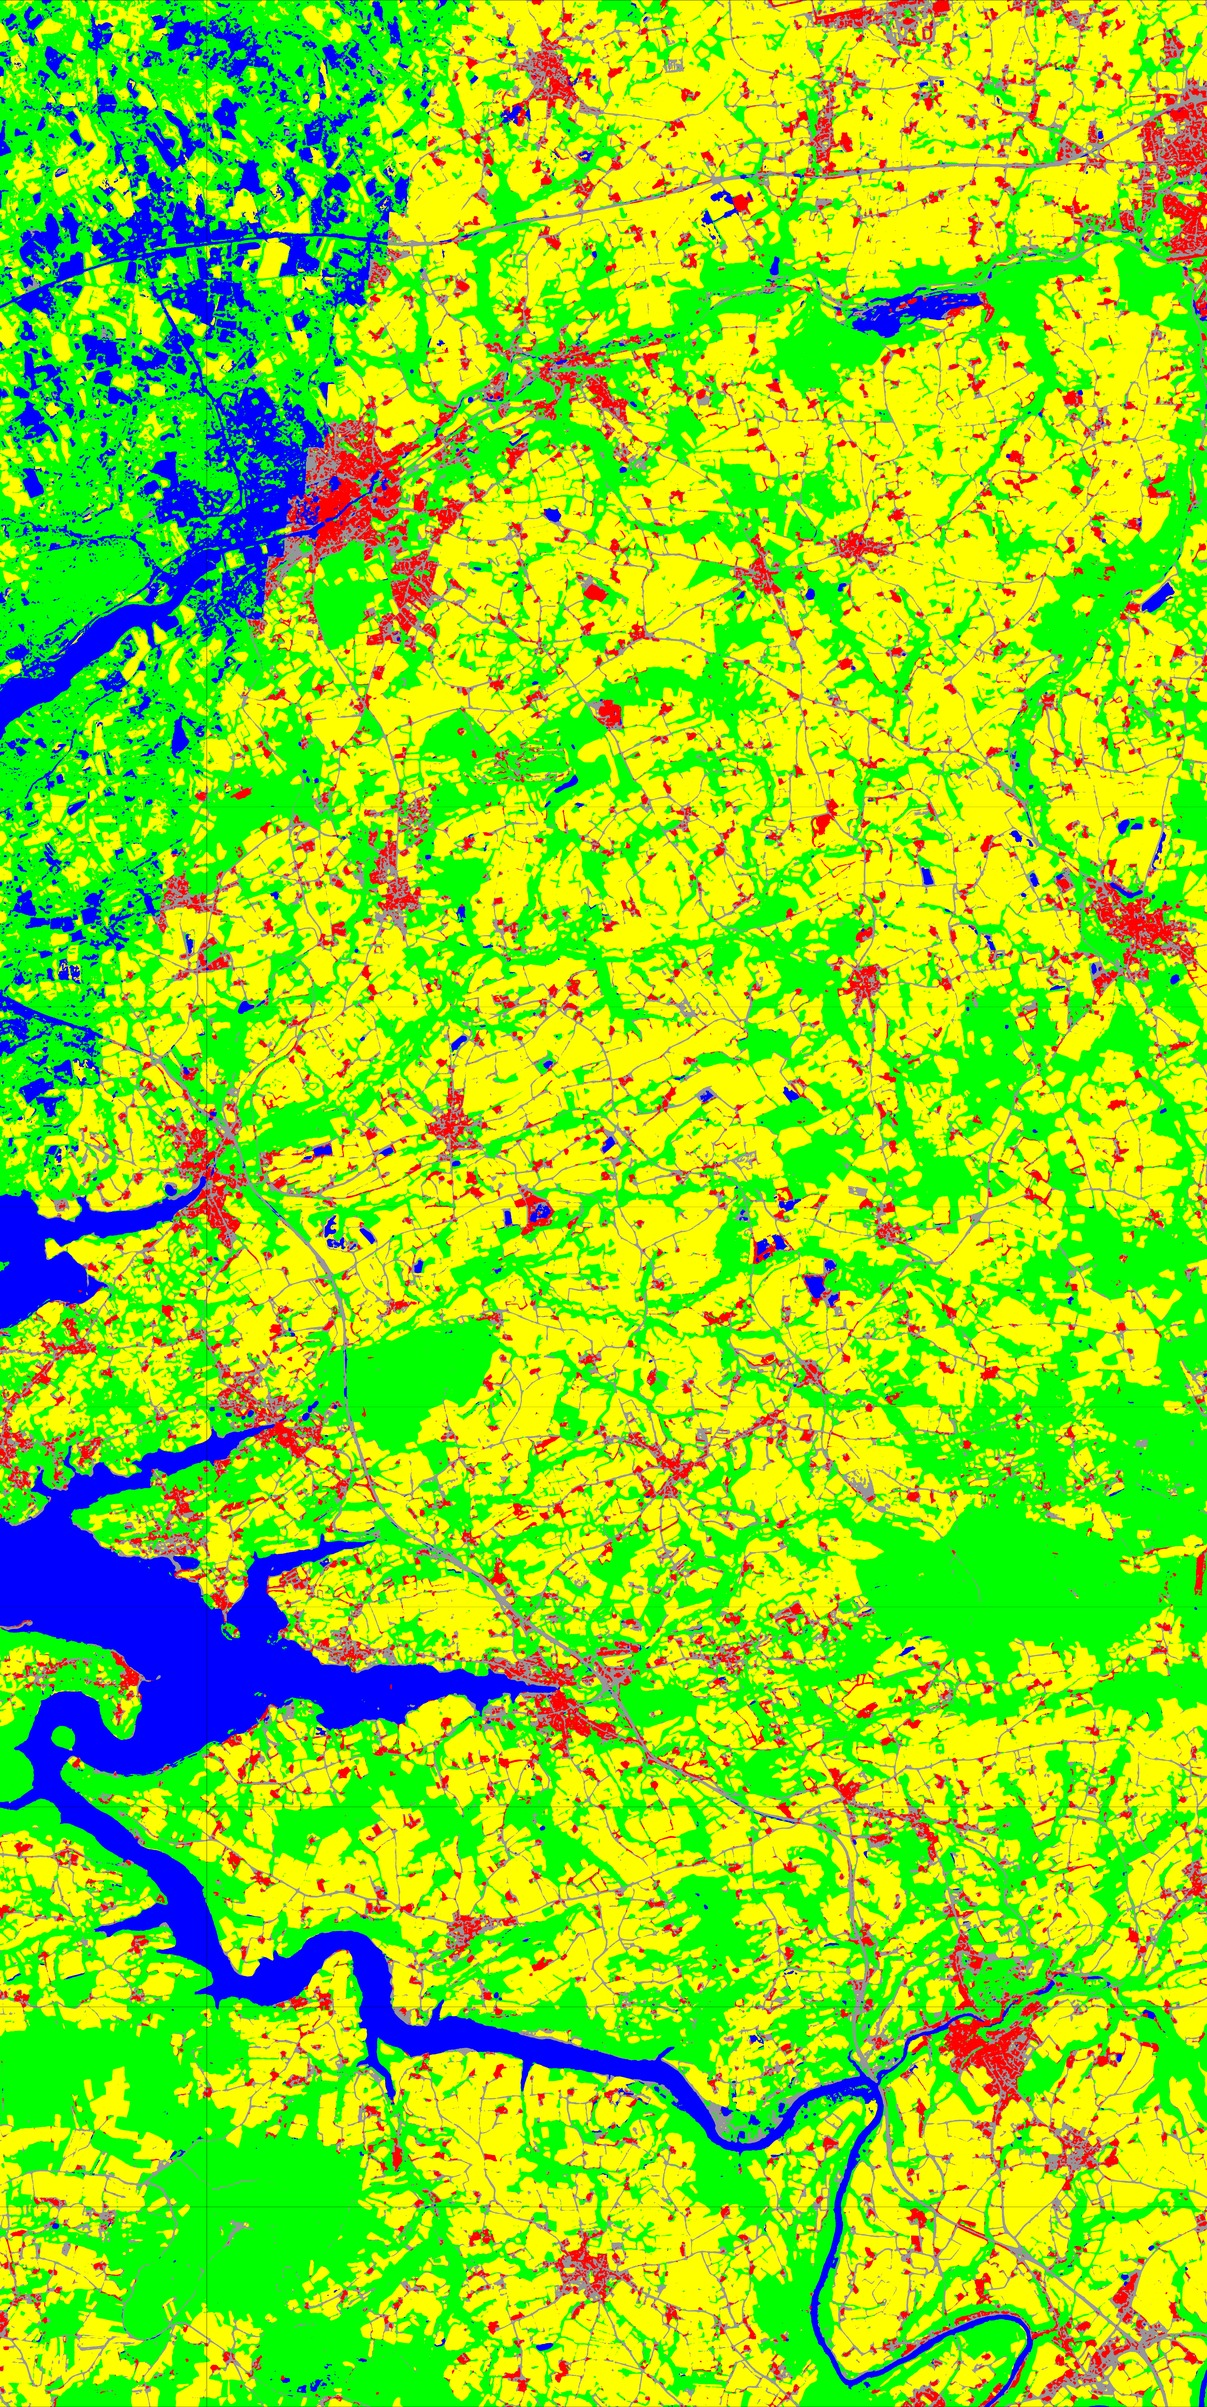
\includegraphics[width=\textwidth]{all_classif_S2}
        \caption{Sentinel-2}
    \end{subfigure}
    \begin{subfigure}{0.49\textwidth}
        \centering
        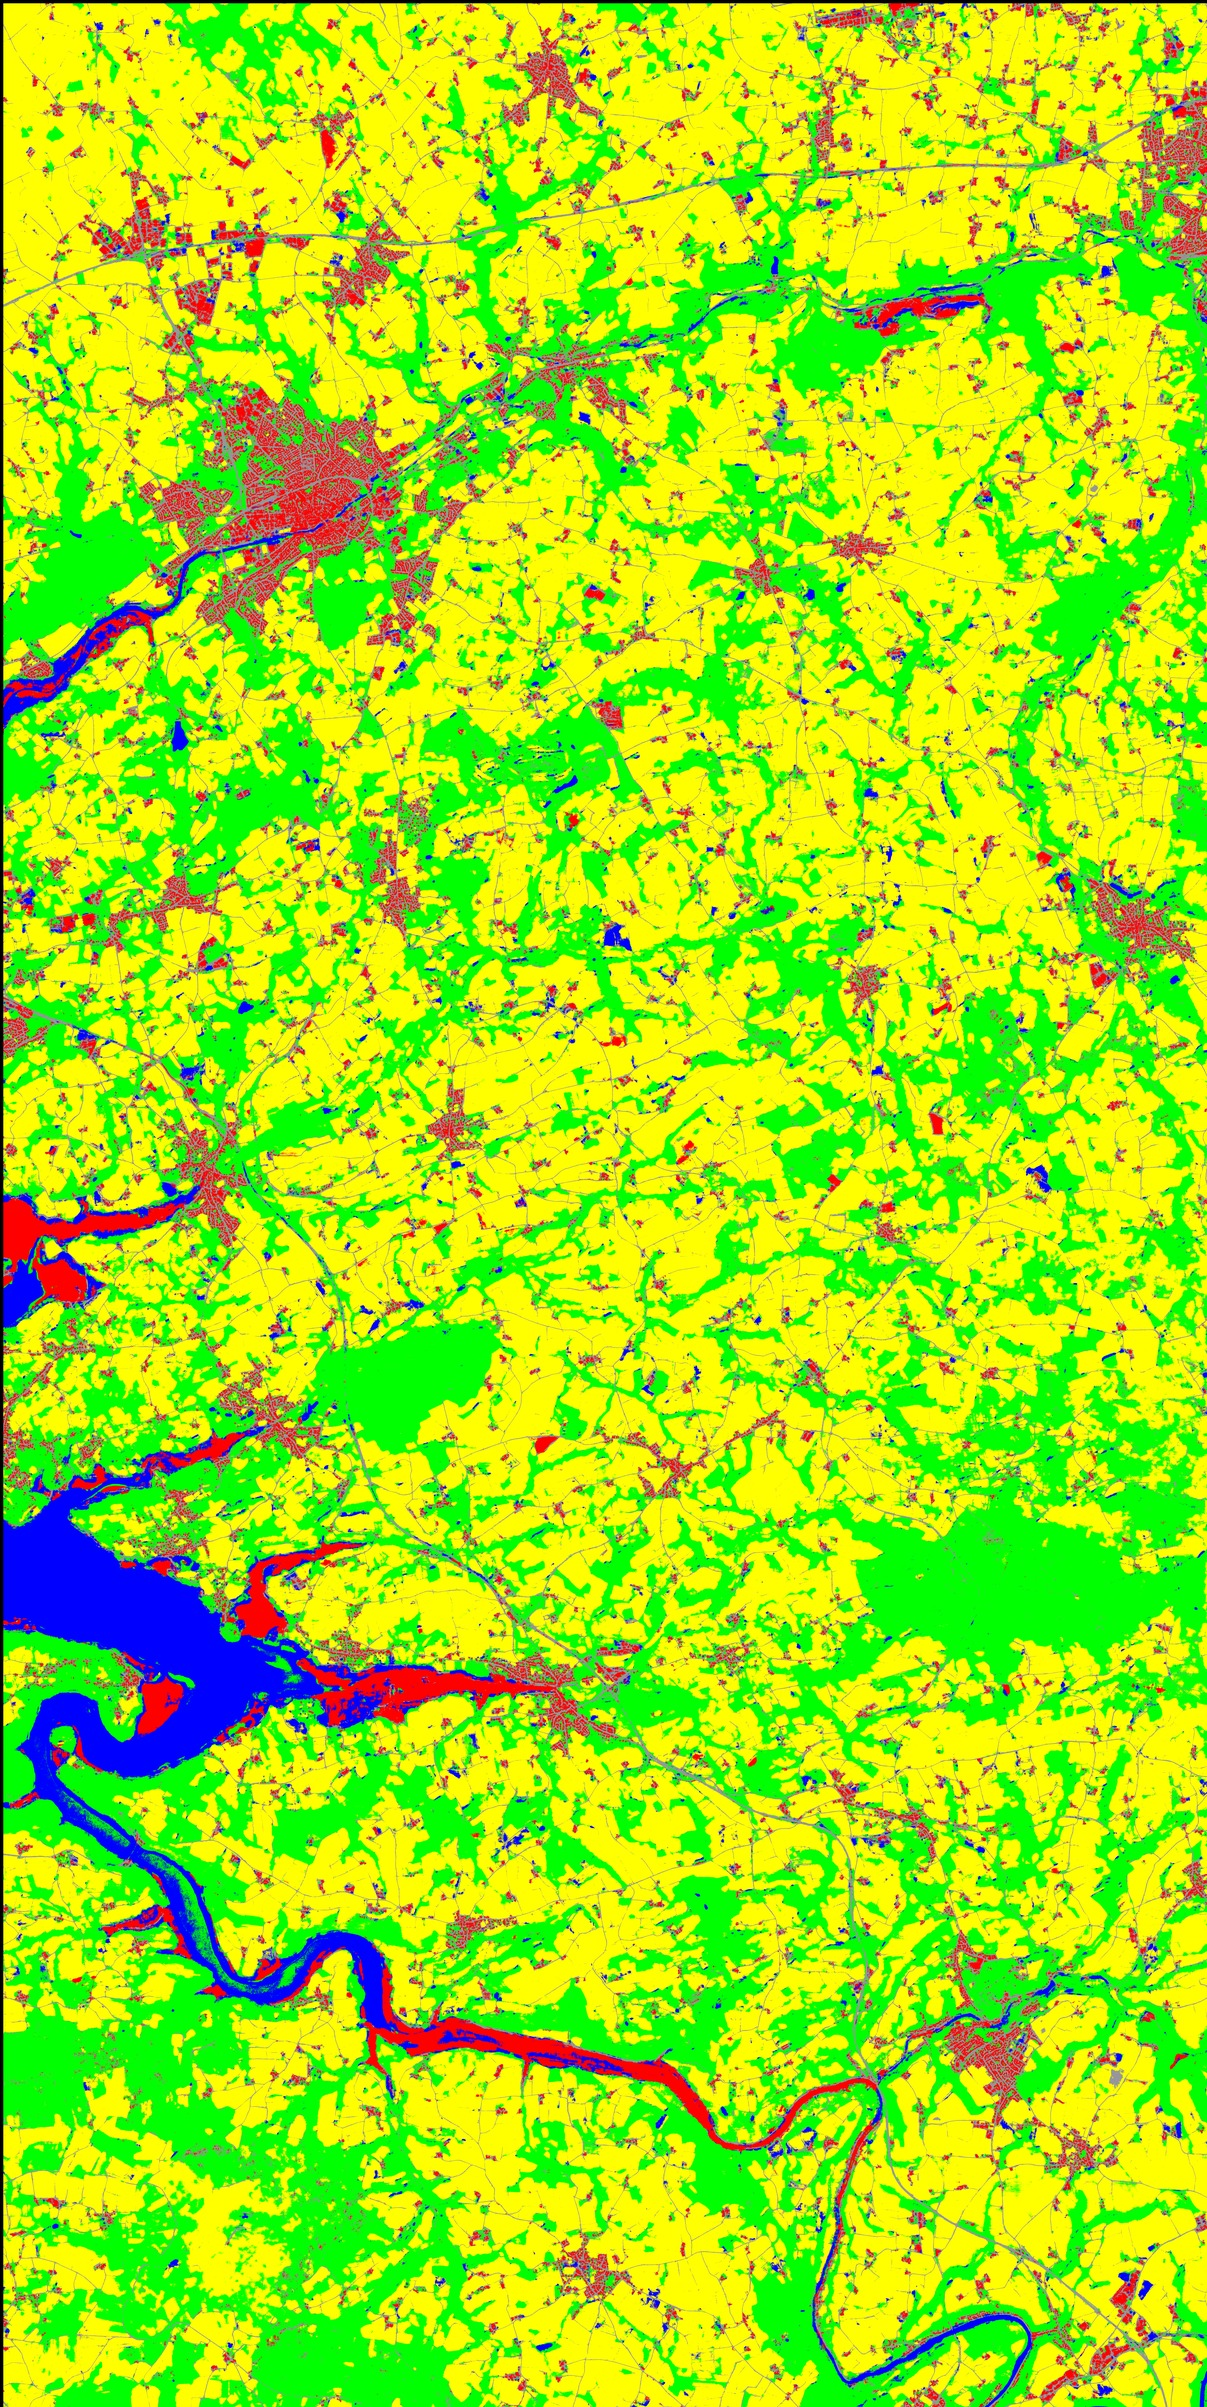
\includegraphics[width=\textwidth]{all_classif_SPOT6}
        \caption{SPOT6}
    \end{subfigure}
    \legende
    \caption{Initial classifications from Sentinel-2 and SPOT 6}
\end{figure}

\begin{figure}[H]
    \centering 
    \begin{subfigure}{0.49\textwidth}
        \centering
        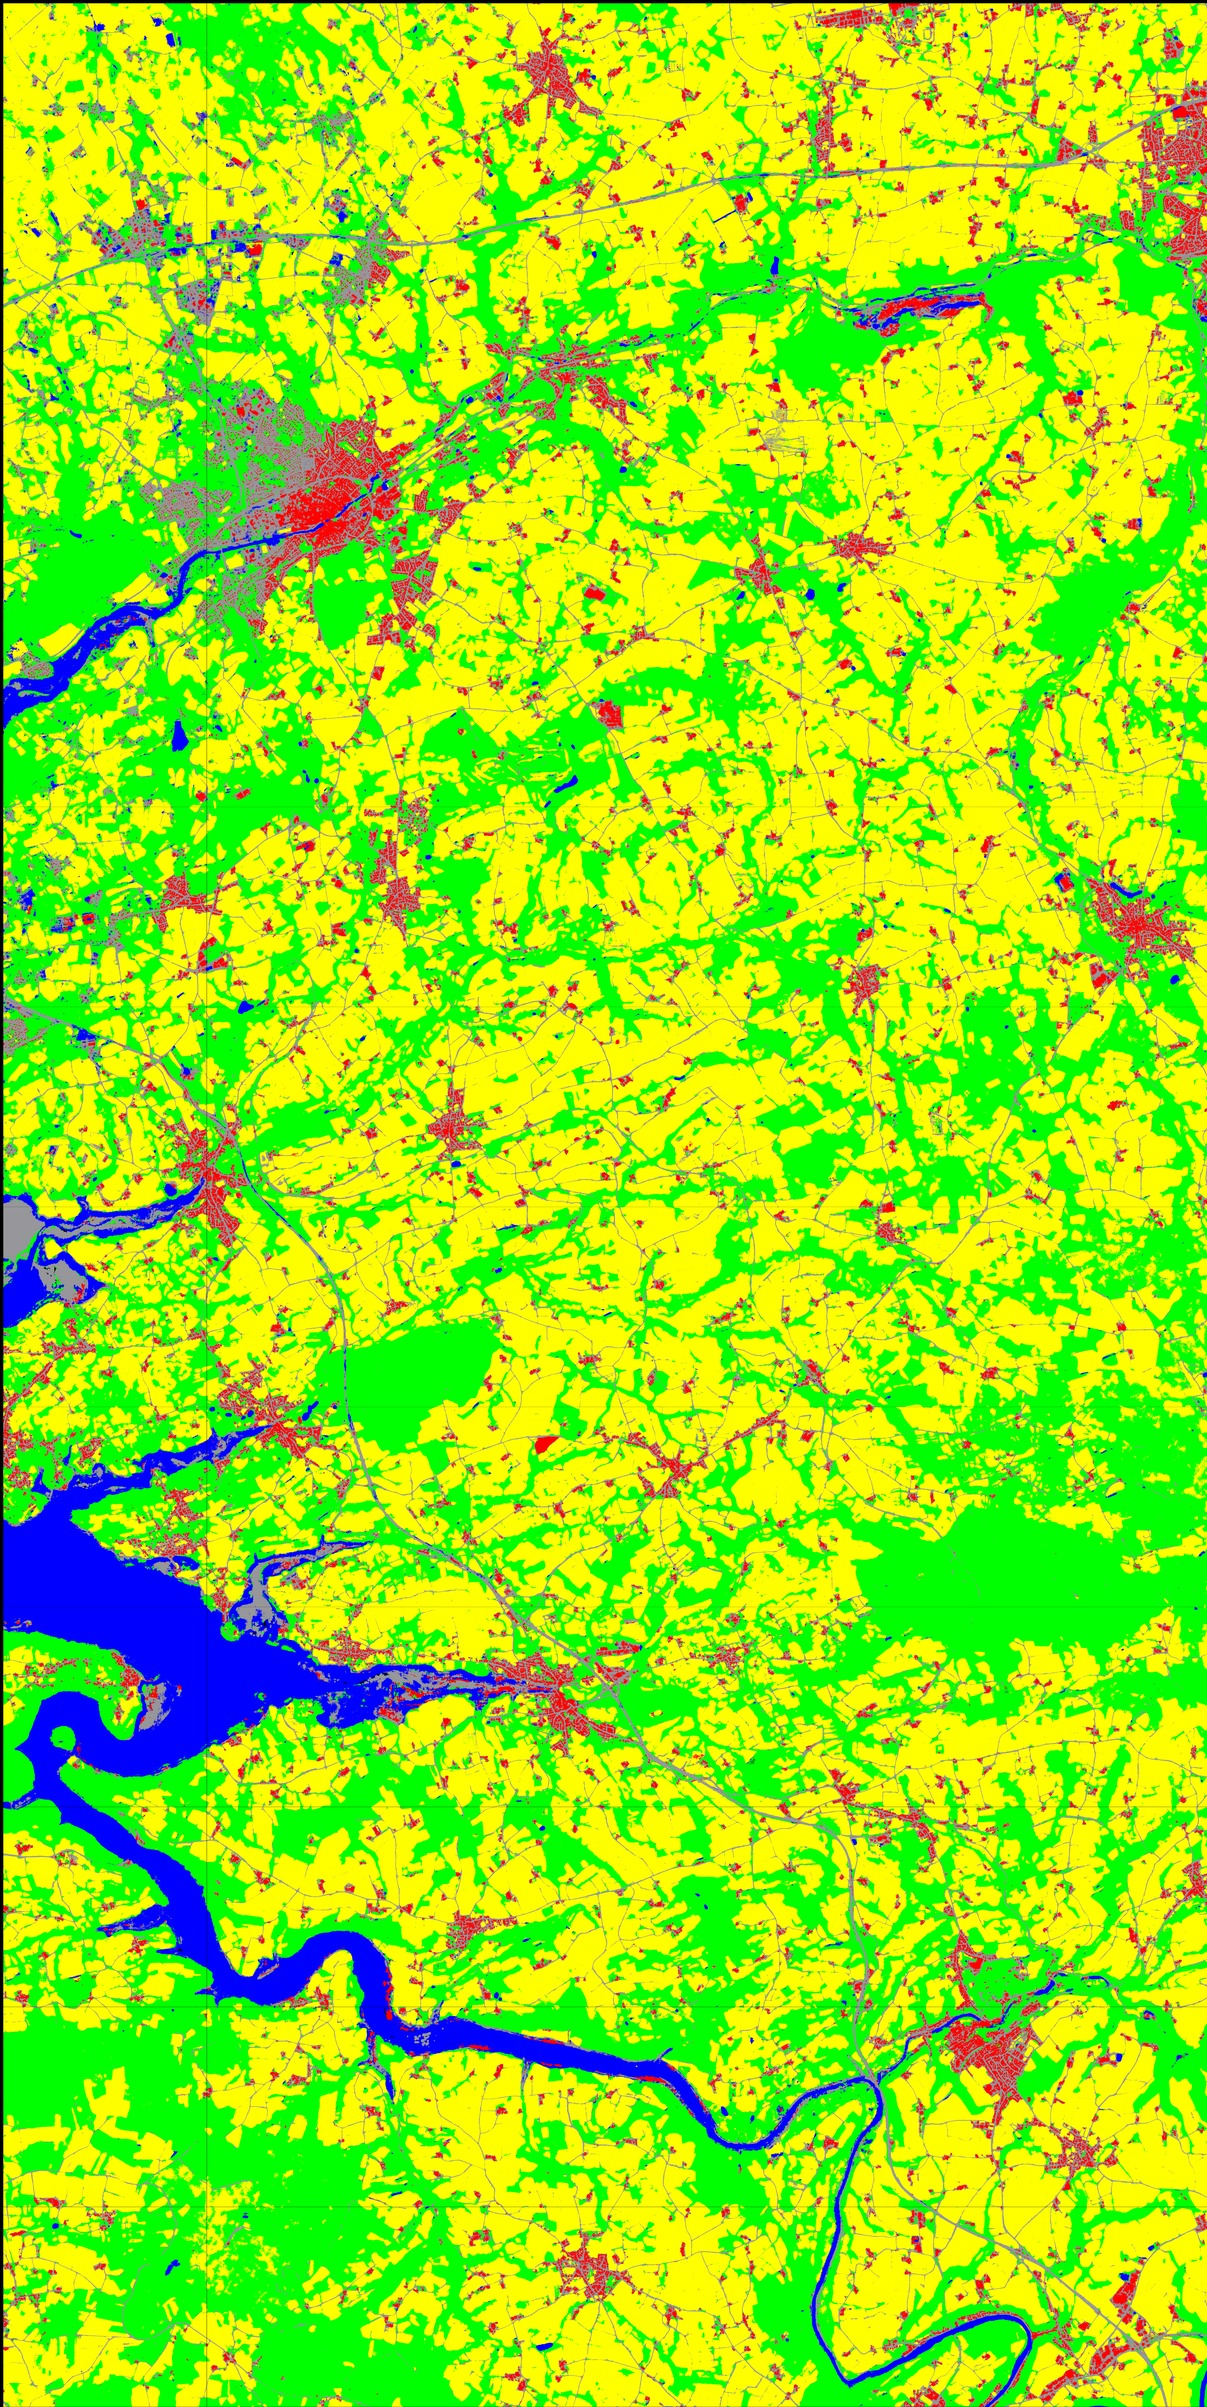
\includegraphics[width=\textwidth]{all_classif_Fusion_Min_weighted}
        \caption{Fusion (Min rule)}
    \end{subfigure}
    \begin{subfigure}{0.49\textwidth}
        \centering
        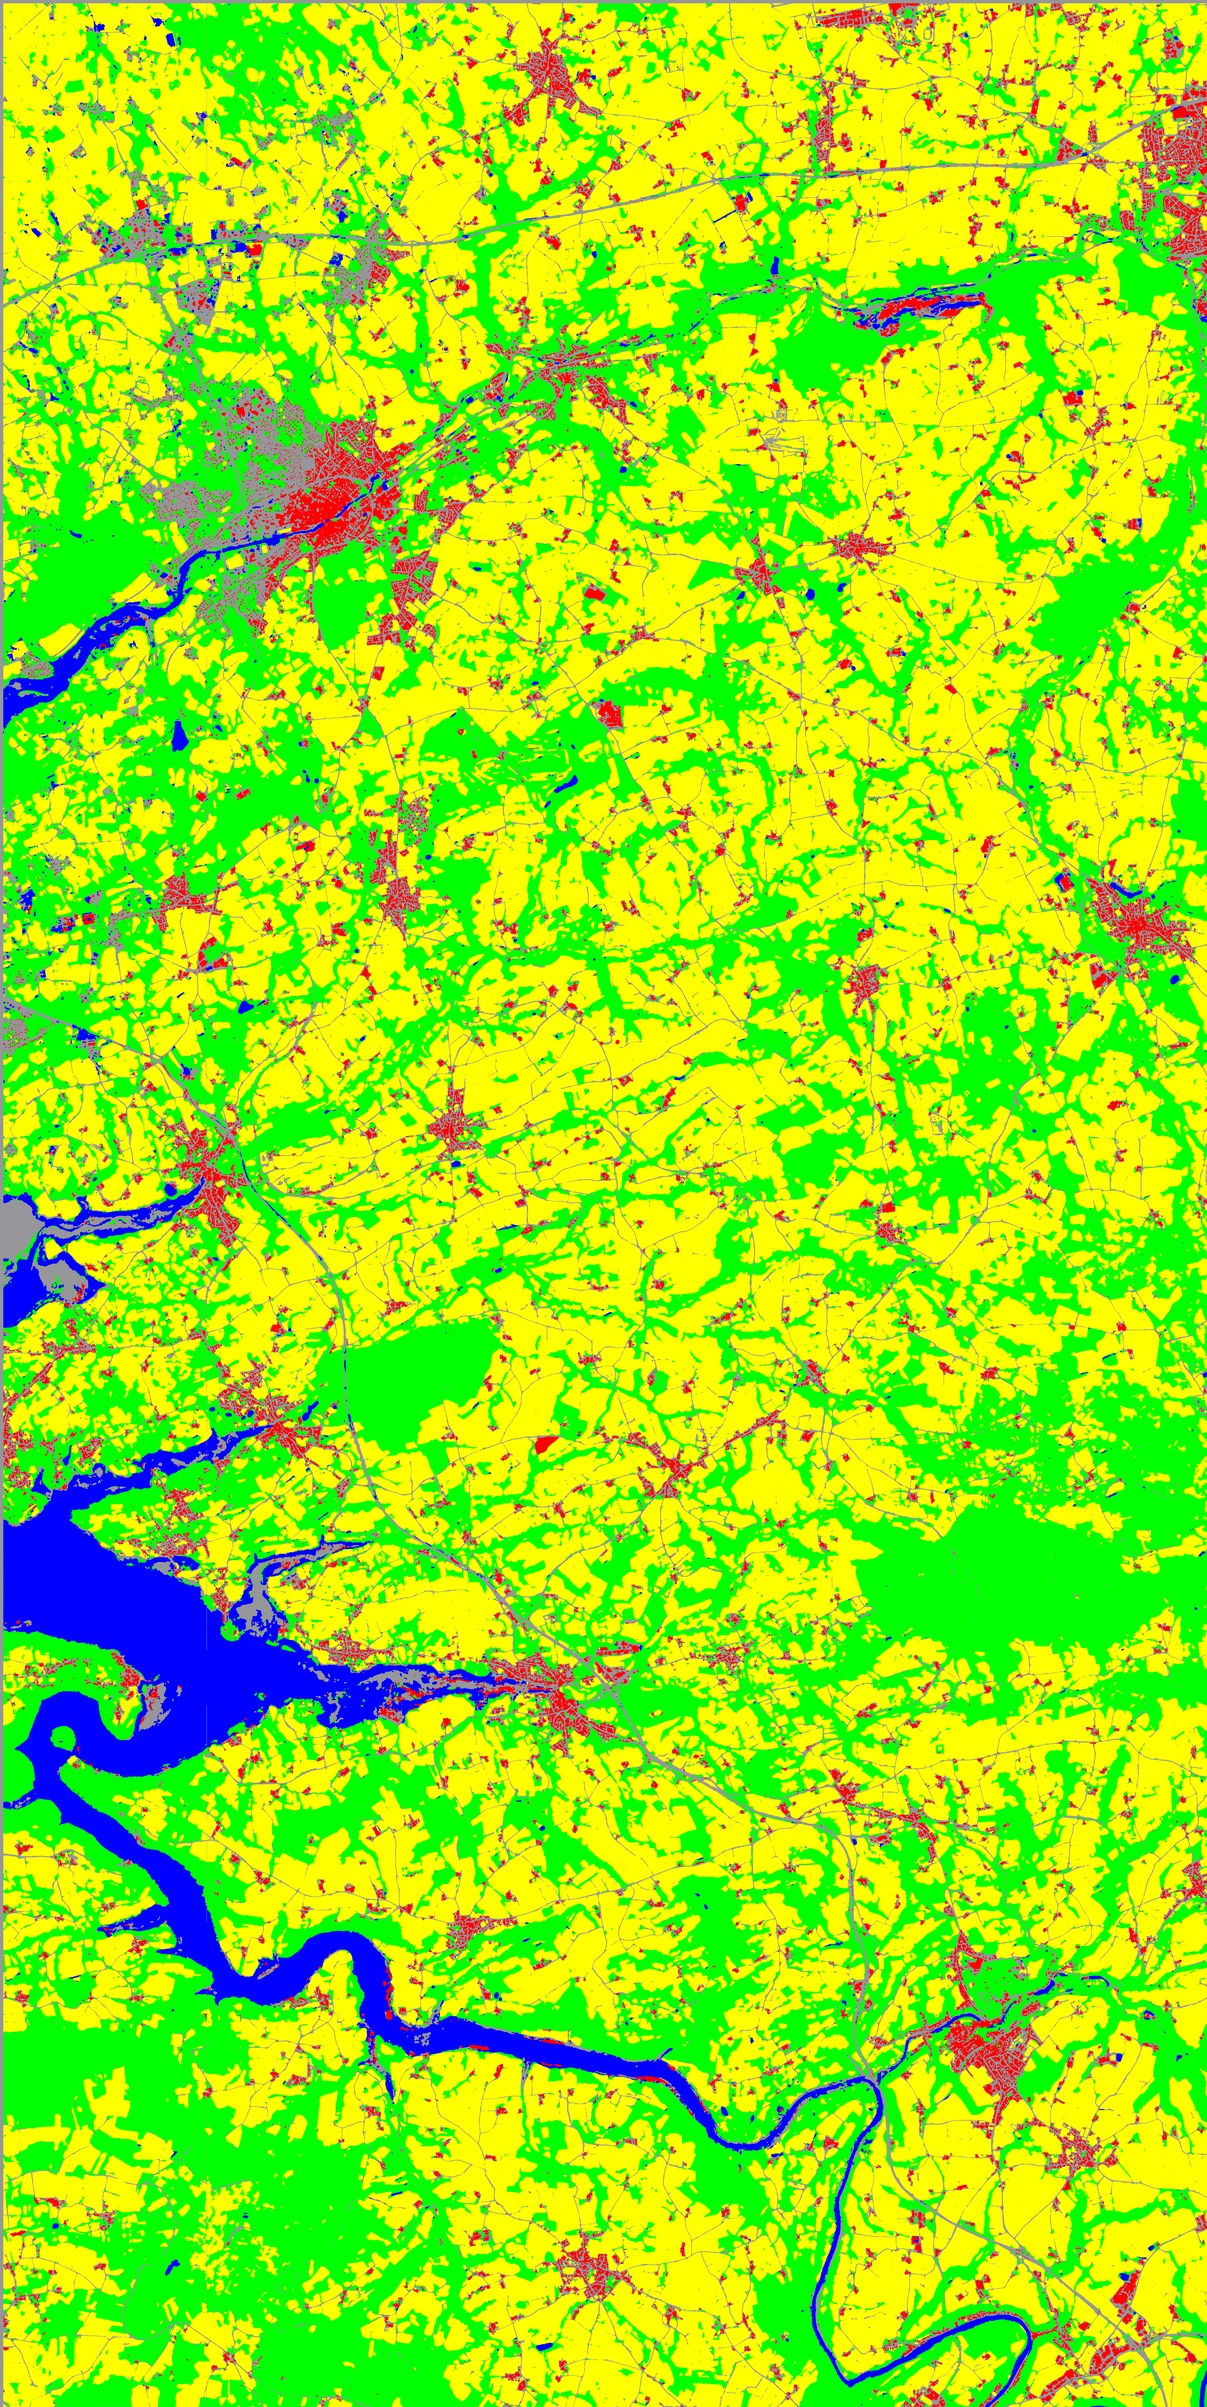
\includegraphics[width=\textwidth]{all_regul_Min_weighted_G2_l1000_g70_e500_0_0_0}
        \caption{Regularization} % parameters
    \end{subfigure}
    \legende
    \caption{Fusion and Regularization}
\end{figure}

\begin{figure}[H]
    \centering 
    \begin{subfigure}{0.49\textwidth}
        \centering
        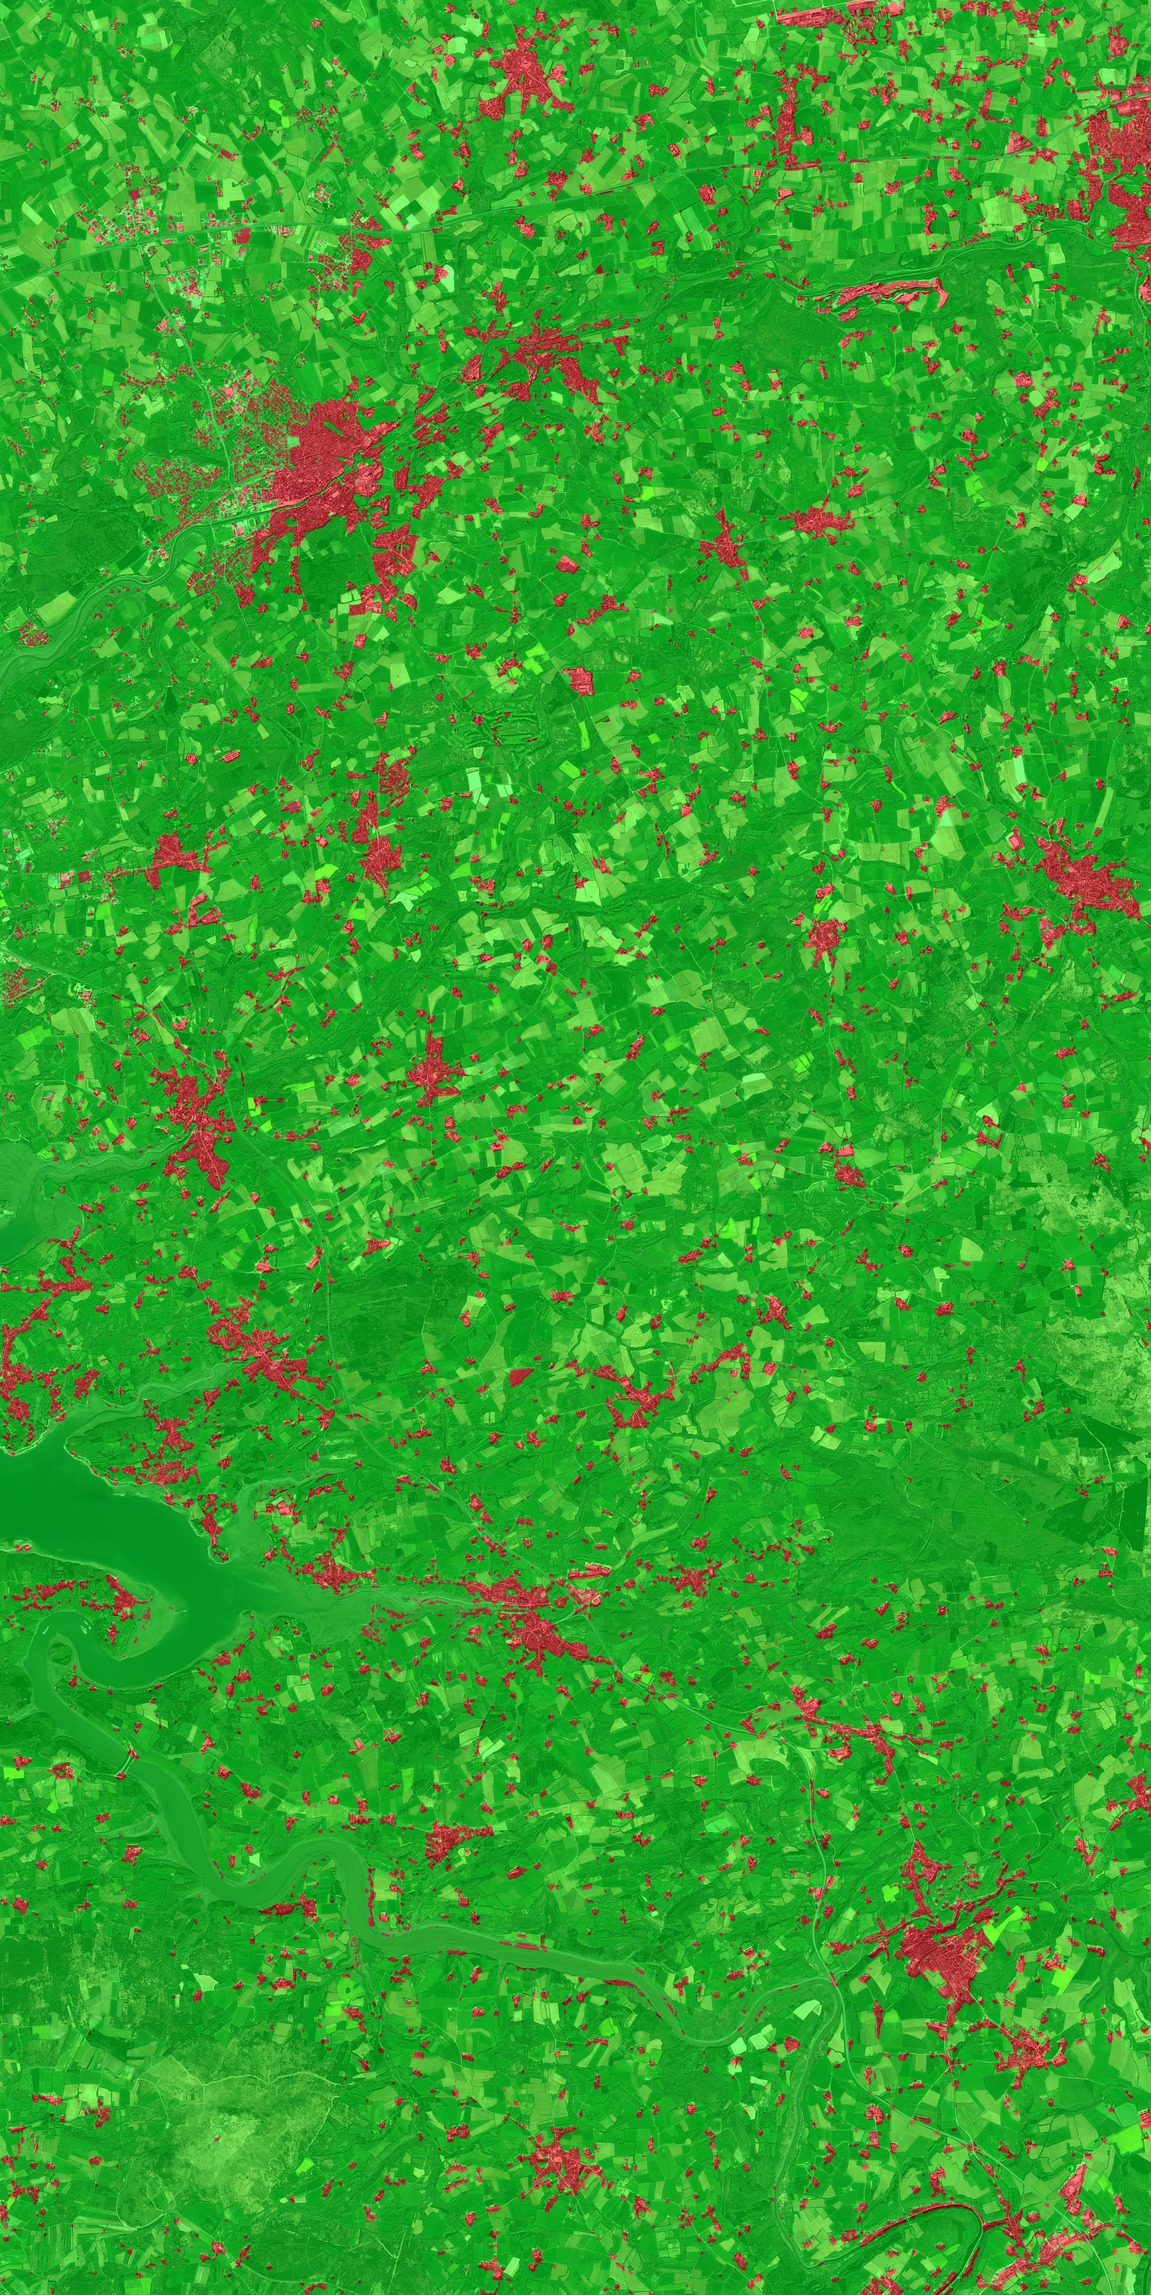
\includegraphics[width=\textwidth]{all_classif_Fusion_Min_overlay}
        \caption{Fusion (Min rule)}
    \end{subfigure}
    \begin{subfigure}{0.49\textwidth}
        \centering
        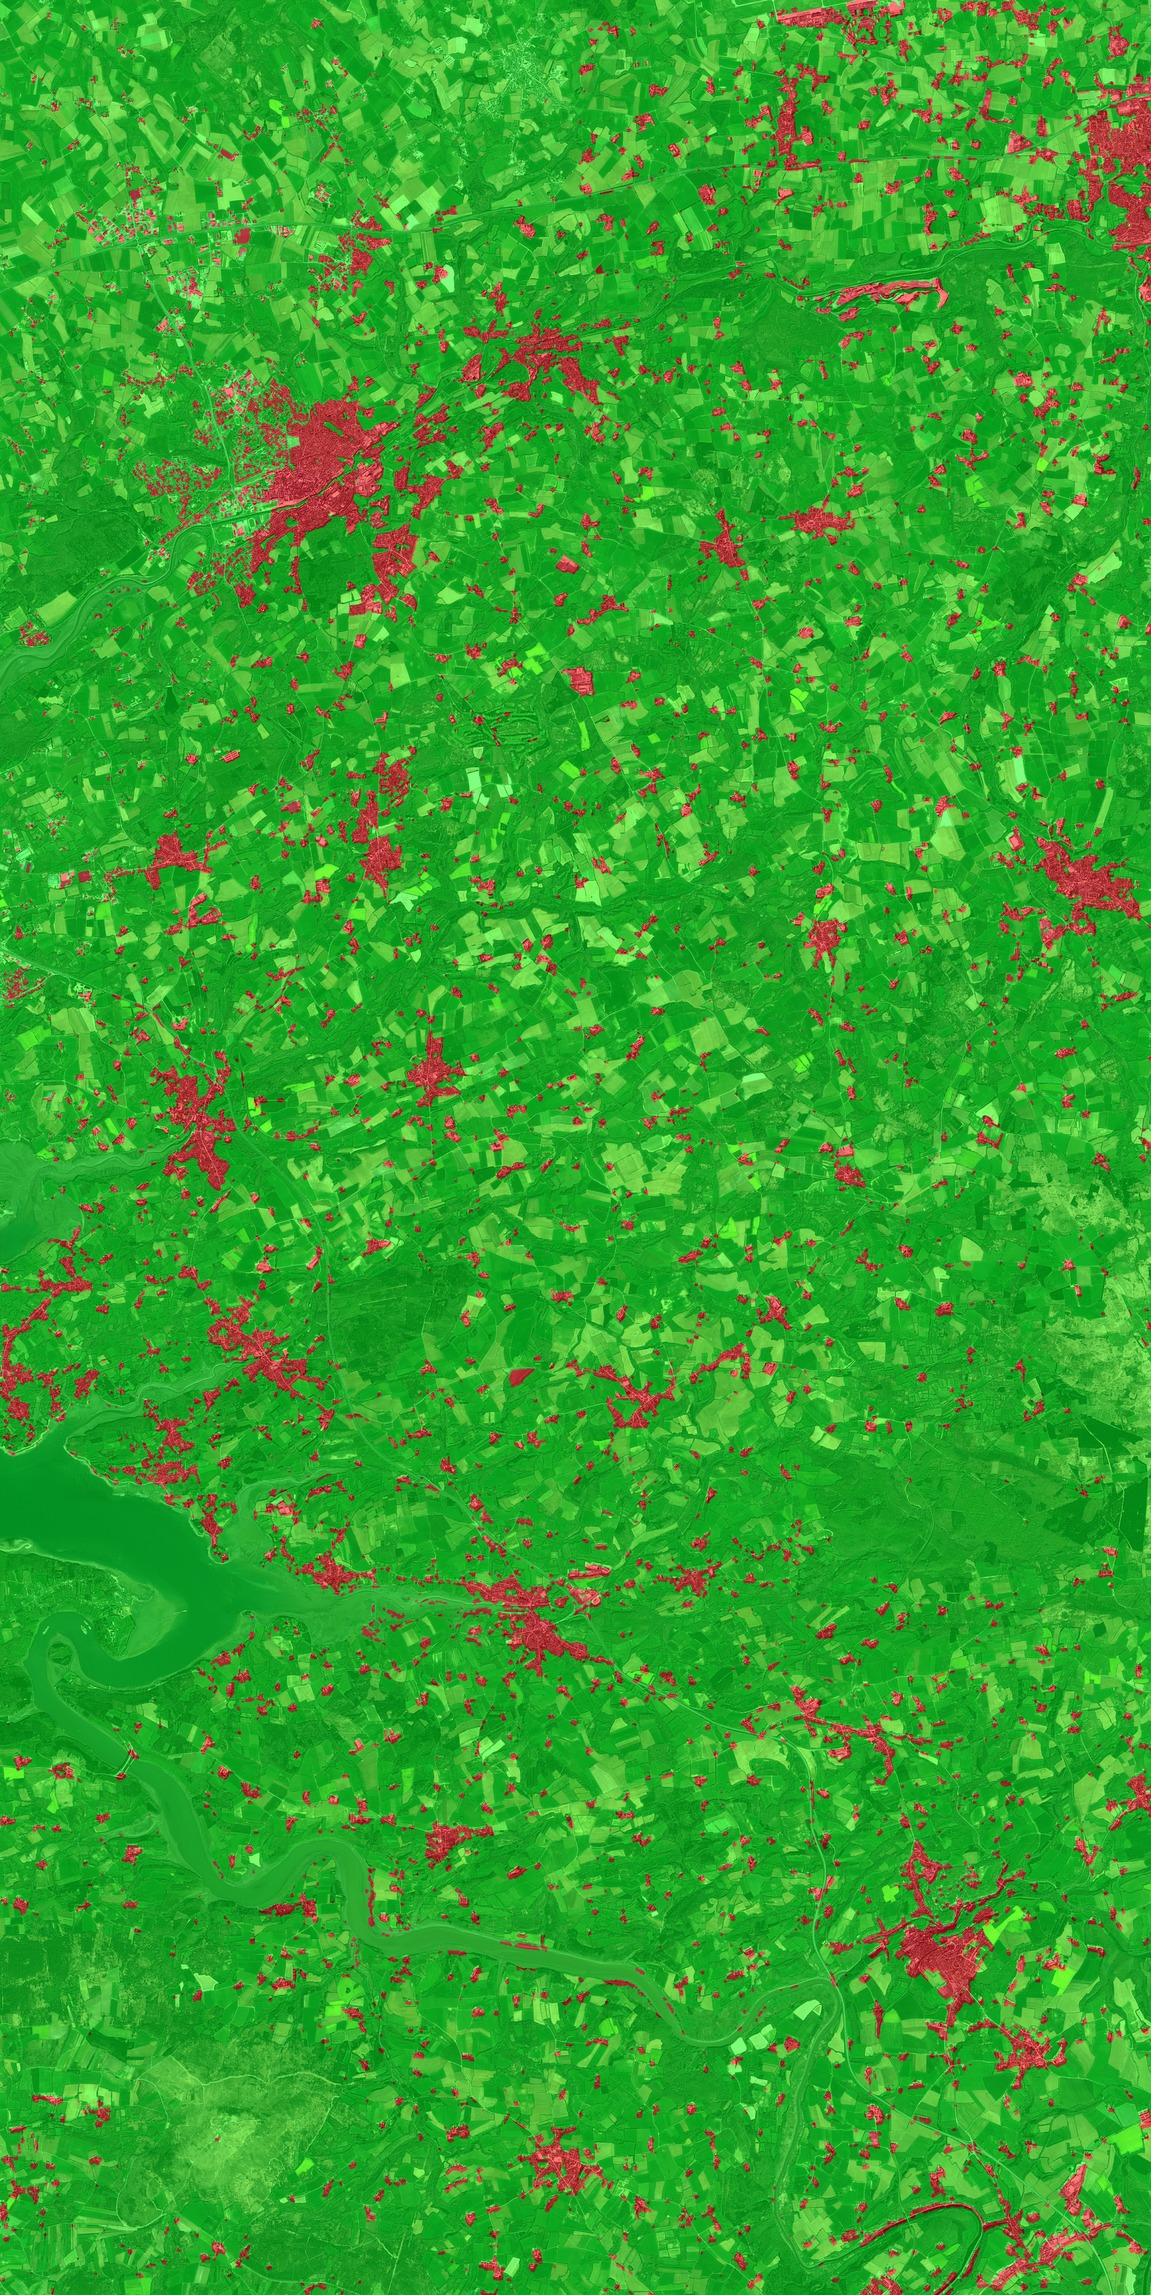
\includegraphics[width=\textwidth]{all_regul_Min_l1000_g30_e500_0_0_0_overlay}
        \caption{Regularization} % parameters
    \end{subfigure}
    \legendebin
    \caption{Second Fusion with S2 and Regularization}
\end{figure}
\begin{figure}[H]
    \centering 
    \foreach \n in {3,8}{
    \begin{subfigure}{0.49\textwidth}
        \centering
        \includegraphics[width=\textwidth]{all_regul_seg_maj_\n_overlay}
        \caption{cut=\n}
    \end{subfigure}
    }
    \legendebin
    \caption{Segmentation and majority vote (I)}
\end{figure}
\begin{figure}[H]
    \centering 
    \foreach \n in {20,30}{
    \begin{subfigure}{0.49\textwidth}
        \centering
        \includegraphics[width=\textwidth]{all_regul_seg_maj_\n_overlay}
        \caption{cut=\n}
    \end{subfigure}
    }
    \legendebin
    \caption{Segmentation and majority vote (II)}
\end{figure}
\restoregeometry
\end{document}
\endinput